\documentclass{article}
\usepackage{graphicx} % Required for inserting images
\usepackage{float}

\title{Analysing Overfitting in Deep Neural Networks}
\author{Divij Khaitan}
\date{\today}
\usepackage{amsmath}
\usepackage{amssymb}
\begin{document}

    \maketitle

    \section{Introduction}
        Deep Neural Networks have revolutionised several fields since their commercial viability was discovered on graphics processing. Today, deeper and deeper networks trained on unfathomably large datasets are ubiquitous in everyday use, even for someone who may not be technically inclined. The increase in the sizes of neural networks does beg the question, how much is too big. Today, OpenAI's GPT-4 model has over a trillion parameters, even though the number of unique sentences it was trained was several orders of magnitude smaller,
        One may rightly investigate the possibility that the model has 'memorised' the training data, rather than 'learning' to recognise patterns in the data as intended. My work intends to possibly establish a framework for analysing whether this has taken place or not.
        \subsection{Related work}
            Every aspect of this topic is well explored, but the field is still in it's nascent stages. Experts do not appear to have consensus on a rigorous definition of what overfitting is, outside of the loose idea of training error dropping alongside test accuracy. \\
            Several author's have tried to test the memorisation capacity of various deep architectures. This is done by scrambling the labels on test data and then looking at the training error. Most deep networks are able to perfectly fit to datasets with even completely random labels, yet we do not see overfitting to this degree in practical situations. \\
            Sanjeev Arora's group has done much work on overparameterisation as well as generalisation error. They have shown there may be tangible benefit to overparameterisation, with regards to both generalisation error as well as rate of convergence. \\
            Soltanolkotabi and Oymak point out benefits to overparameterisation in the same vein. They showed that the training error is low and the network parameters remain 'close' to the initialised values with sufficient overparameterisation. They additionally proved that it also gives the model some resistance to labels being corrupted. \\
            There has been some work similar to mine in the field of explainability. SUMMIT identifies important neurons in intermediate layers and relationships between these important neurons, analysing the resulting network of neurons to identify the features recognised by different layers of the network. Neural Activation Patterns (NAP) examines neural activation patterns and tries to cluster intermediate activations to attribute the recognition of various patterns to particular portions of a particular layer of a neural network. \\

    \section{Characterisation of Input Distributions in terms of Neuron Activations}
        Shifts in distribution are situation when the distributions of the training and testing sets are not identical. In literature, the most common classification of these shifts are concept shift and covariate/data shift. \\

        \textbf{Covariate Shift} is when $p(x)$ changes, but not $p(y|x)$, i.e. the inputs change but the labels stay the same. An example would include training a model on voting patterns for India, and testing the model on voting patterns from China. \\
        
        \textbf{Concept Shift} is when $p(x)$ remains the same, but $p(y | x)$ does not. This can be thought of as training on a similar dataset with slightly different labels. An example would be training a model to issue red alerts for storms in Delhi, and testing it to issue red alerts in Pune. While both cities might see similar rainfall patterns, they may be equipped very differently to handle the same amount of precipitation. \\

        Detecting such shifts can be difficult in practice, because the distributions themselves cannot be categorised easily. Our hypothesis is that in CNNs, the neurons from the fully connected layers should have similar activation patterns across the same classes, and thus we should be able to attach distributions of neuron activations to each class, which should be sensitive to a shift in the distribution of inputs. \\
        
    \section{Class-wise Frequencies of Neuron Activations}
        For this section, we analysed the outputs of each fully connected hidden layer, i.e. for a network $f = \phi_{n}(f_{n}(\dots(\phi(f_1(x)))))$, we analysed $x_k = \phi(f_{k}(\dots(\phi(f_1(x)))))$. Alexnet in particular is RELU-activated with the exception of the final layer, so $\phi_i = \text{ReLU} \text{ if } i < n \; \sigma(x) \text{ if } i = n$. We utilised the following definitions of significance \\
        \[S_1(x_{i}) = 1 \text{ if } x_i > 0\] 
        \[S_2(x_{(i)}) = 1 \text{ if } \frac{x_{(i)}}{x_{i+1}} > \epsilon\] 
        $x_{(i)}$ denotes the i$^\text{th}$ order statistic. The first definition is comes from the ReLU activation, where a neuron is considered 'active' if it is positive. The justification for the second is the assumption of a high signal to noise ratio, where smaller activations correspond to noise while larger activations correspond to meaningful information. Practically, we set the value of $\epsilon$ to be 1000. We computed the proportions of every neuron activating in any given class under both definition, and the results are attached below. Each neuron has a proportion of activations for each class in between 0 and 1, we have displayed histograms of the number of neurons in 100 bins for different activation proportions. Below is the result for a particular class under both $S_1$ and $S_2$. The y-axis is the number of neurons in each bin, and the x-axis has the bins of different proportions of activation across all the images in the class. This shows a move towards sparsity in activation with an increase in depth.
        \begin{figure}[H]
            \centering
            \begin{minipage}{0.45\textwidth}
                \centering
                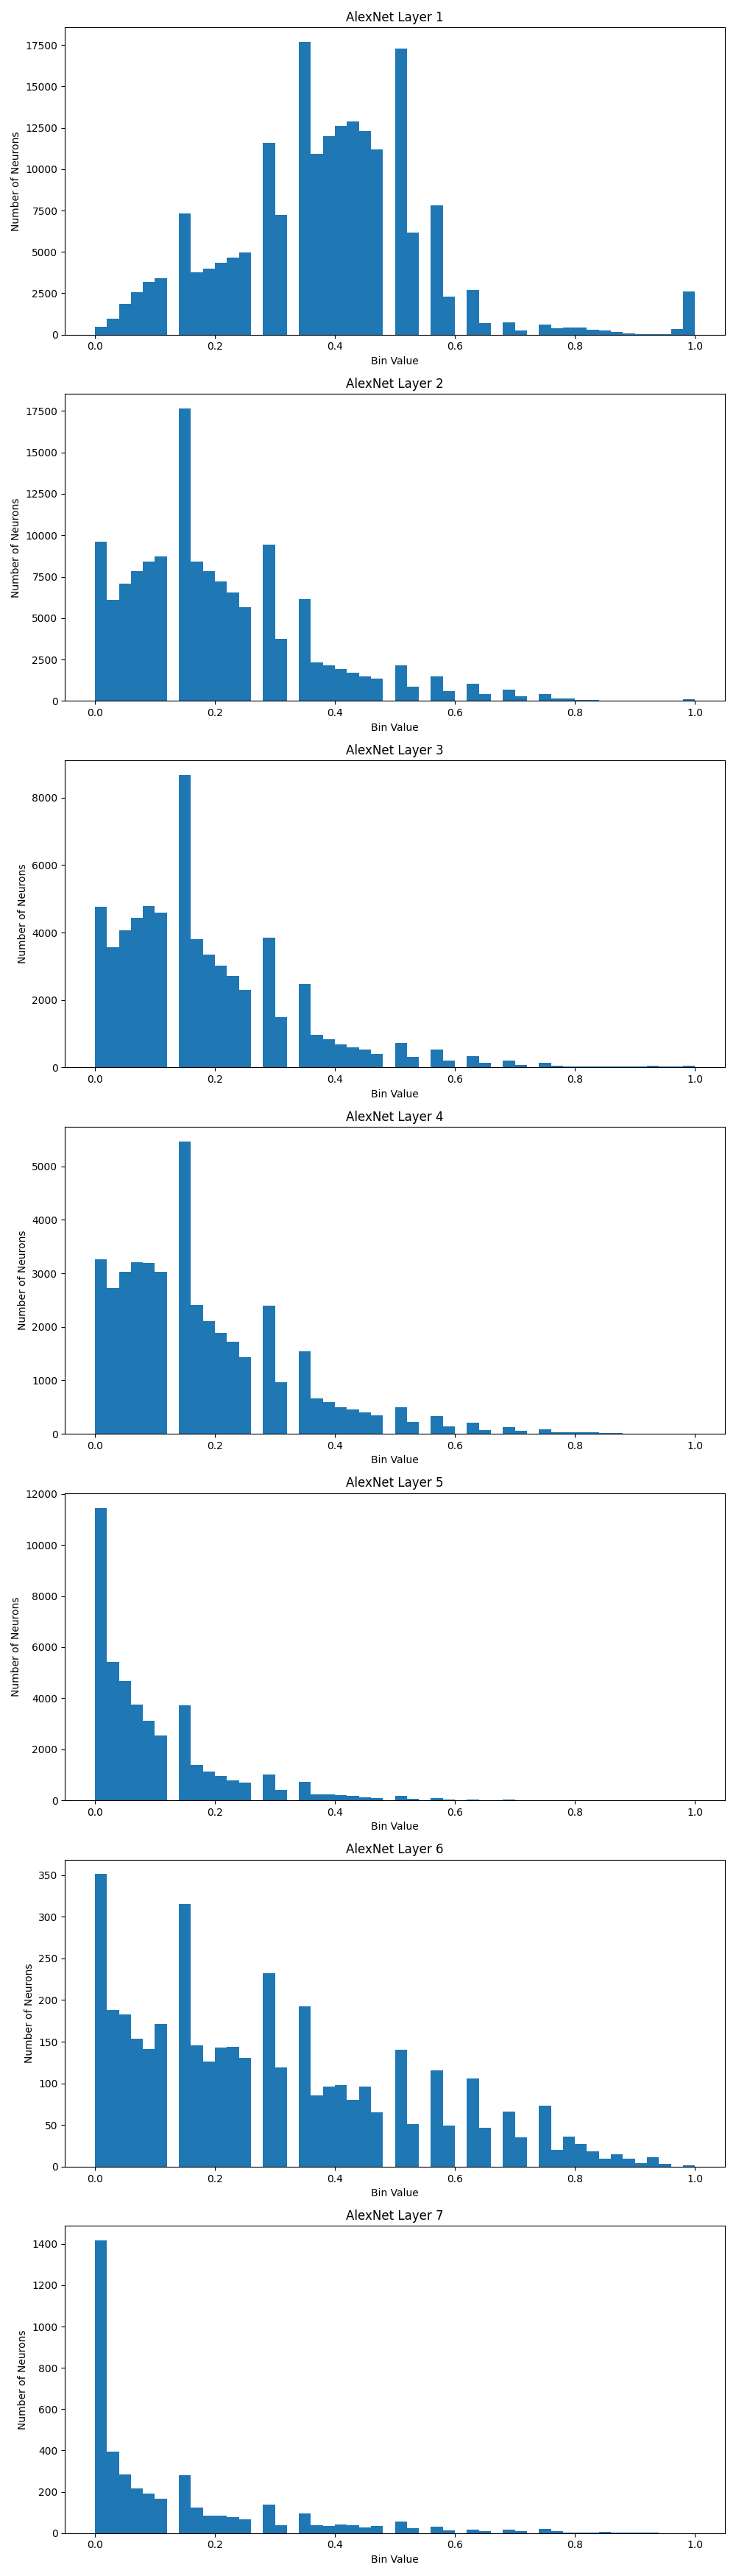
\includegraphics[width=\textwidth]{images/alexnet_class_frequency_list_n01601694.png} % first image
                
            \end{minipage}\hfill
            \begin{minipage}{0.45\textwidth}
                \centering
                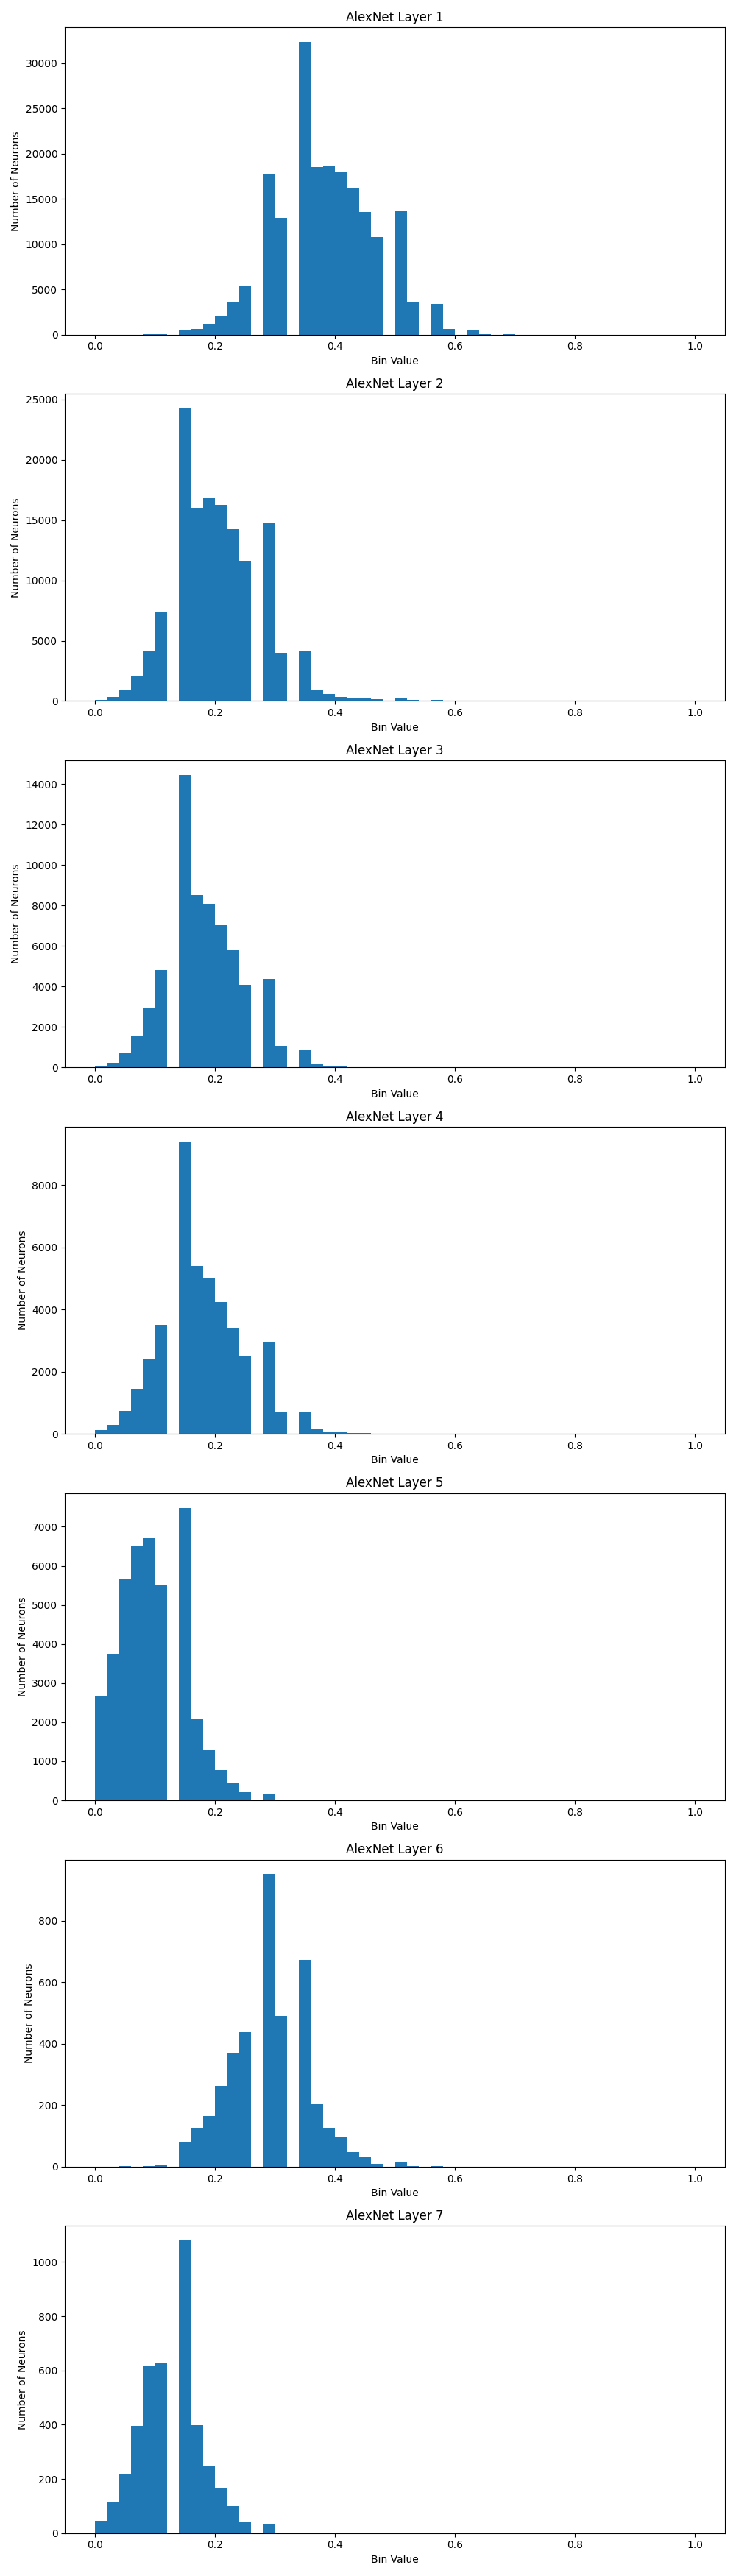
\includegraphics[width=\textwidth]{images/alexnet_class_frequency_list_threshold_n01601694.png} % second image
            \end{minipage}
            \caption{Histograms for AlexNet activations under $S_1$(left) and $S_2$(right). There is a distinct clustering towards the left inside the convolutional layers (plots 1 to 5) and then inside the fully connected layers as well (plots 6 and 7)}
            \label{fig:neuron_activation_frequency}
        \end{figure}

        % \begin{figure}[ht]
        %     \centering
        %     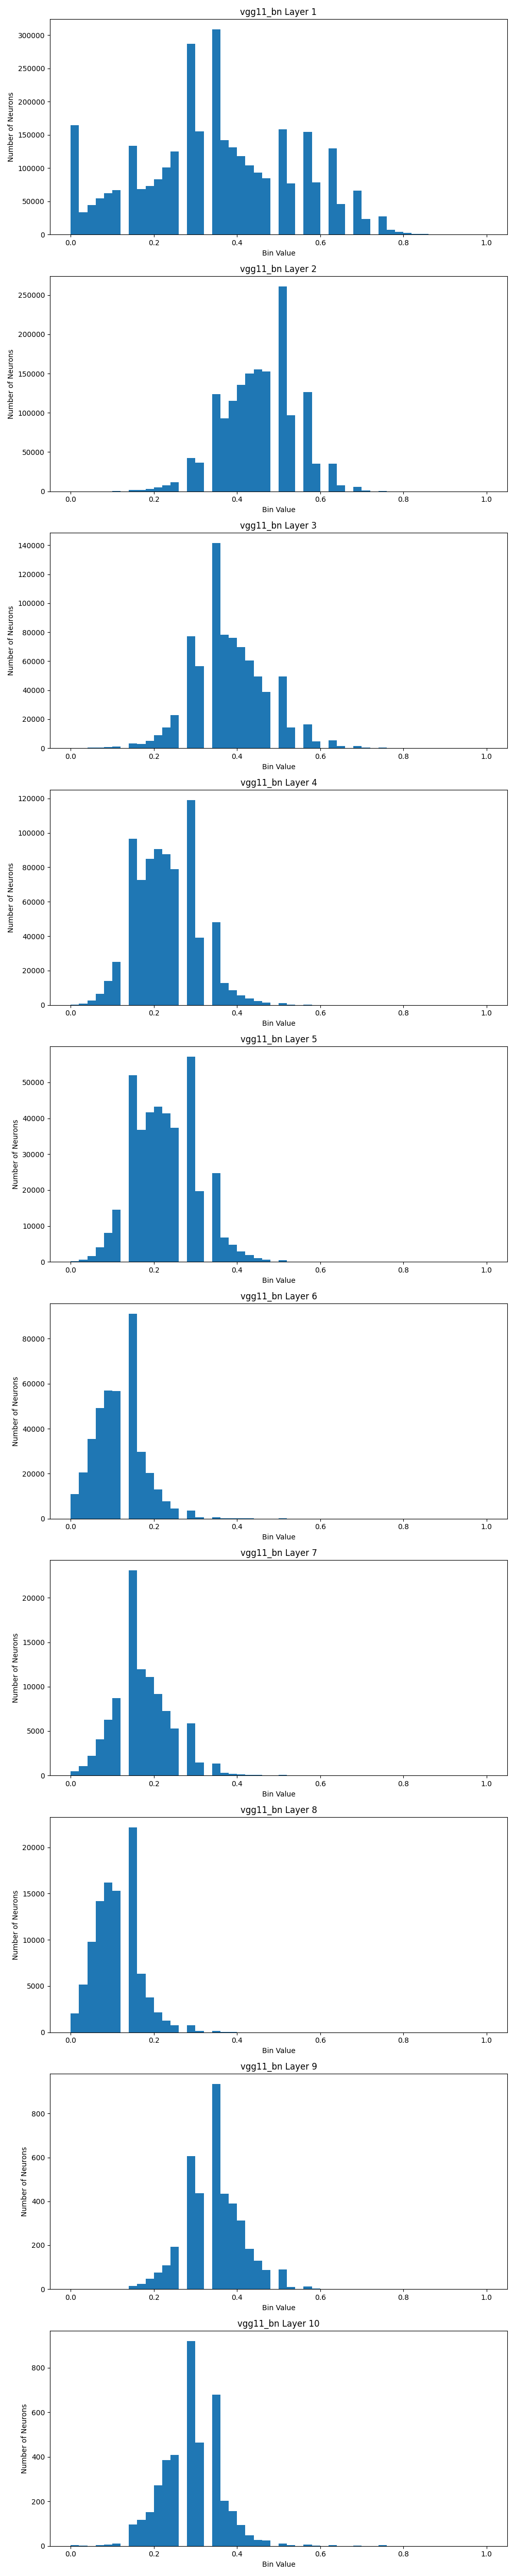
\includegraphics[height=\textheight,keepaspectratio]{vgg11_bn_class_frequency_list_n01601694.png}
        %     \caption{Histogram for VGG11 with thresholding. We observe the same behaviour here}
        %     \label{fig2}
        % \end{figure}
    \section{Class-wise Patterns of Neuron Activations}
        We also plotted the proportion of successes of each neuron in each layer. Some of the results for the final layer of different classes are attached below. The key takeaway is once again the sparsity of the activations, with most neurons having small activations and a few neurons having large activations. For ease of viewing, the vectors were ravelled to form a rectangle with approximately equal sides. Below attached are results from the final 2 layers of a single class.
        \begin{figure}[H]
            \centering
            \begin{minipage}{0.45\textwidth}
                \centering
                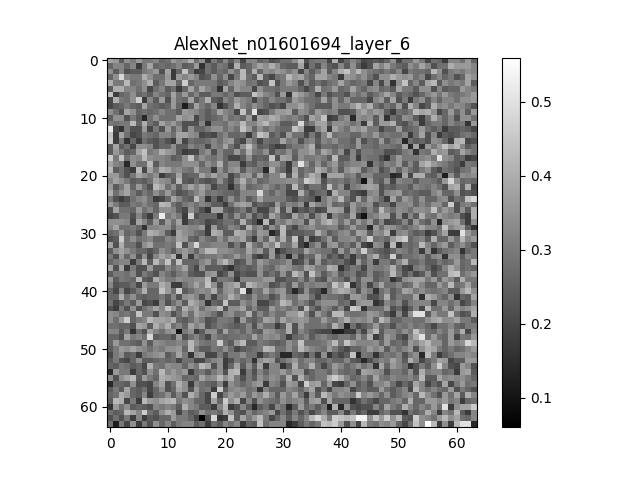
\includegraphics[width=\textwidth]{images/AlexNet_n01601694_layer_6.png} % first image
                
            \end{minipage}\hfill
            \begin{minipage}{0.45\textwidth}
                \centering
                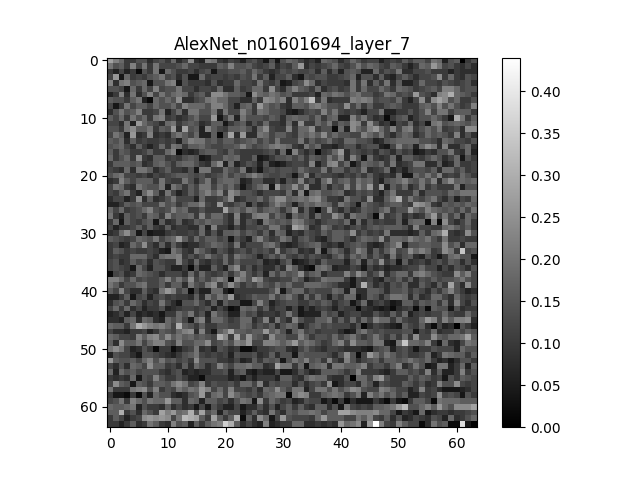
\includegraphics[width=\textwidth]{images/AlexNet_n01601694_layer_7.png} % second image
            \end{minipage}
            \caption{Activation proportions of neurons for the fully connected layers 6 and 7 of alexnet}
            \label{fig:neuron_activation_pattern}
        \end{figure}
        
    \section{Entropies in Between Classes}
        
    \section{Class-Wise Frequencies of Significant Neuron-Weight Interactions}
    As an additional approach, we decided to study the interactions in a neural network at a more granular level. Instead of just looking at the final value of the neuron, we decided to look at each individual weight being multiplied into each neuron. In this case, what we did is described below. \\
    The final layer of the neural network operates as follows. Given an activation vector $x \in \mathbb{R}^{n_{in} \times 1}$ and a weight matrix $W \in \mathbb{R}^{n_{out} \times n_{in}}$ \\
        \[
            \begin{bmatrix}
                w_{1,1} & \dots & w_{1,n_{in}} \\
                \vdots & \ddots & \vdots \\
                w_{n_{out}, 1} & \cdots & w_{n_{out}, n_{in}} \\
            \end{bmatrix}
            \begin{bmatrix}
                x_1 \\
                \vdots \\
                x_{n_{in}} \\
            \end{bmatrix}
            = 
            \begin{bmatrix}
                w_{1,1}x_1 + w_{1, 2}x_2 + \dots + w_{1, n_{in}}x_{n_{in}} \\
                \vdots \\
                w_{n_{out},1}x_1 + w_{n_{out}, 2}x_2 + \dots + w_{n_{out}, n_{in}}x_{n_{in}}
            \end{bmatrix}
        \]
        This would not allow us to study the individual activation-weight pairs, because they would all be summed up. A vector operation that computes the sum over the rows of a matrix is postmultiplication by the all 1s vector, so by factoring out this vector we can get the required information. Factoring out the all 1s vector from the neurons in the penultimate layer, we get an diagonal matrix with the neurons activations as entries \\
        \[
            \begin{bmatrix}
                w_{1,1} & \dots & w_{1,n_{in}} \\
                \vdots & \ddots & \vdots \\
                w_{n_{out}, 1} & \cdots & w_{n_{out}, n_{in}} \\
            \end{bmatrix}
            \begin{bmatrix}
                x_1  & \dots & 0 \\
                \vdots & \ddots & \vdots \\
                0 & \dots & x_{n_{in}} \\
            \end{bmatrix}
            = 
            \begin{bmatrix}
                w_{1,1}x_1  & \dots & w_{1,n_{in}}x_1 \\
                \vdots & \ddots & \vdots \\
                w_{n_{out}, 1}x_{n_{in}} & \dots & w_{n_{out}, n_{in}}x_{n_{in}} \\
            \end{bmatrix}
        \]
    The definition of significance we decided on was 
    \[S(x_{ij}) = 1 \text{ if } \frac{x_{ij}}{\sum_j x_{ij}} > \frac{1}{n_in} \]
    The justification behind this is the idea that if an activation is of an above average proportion of the final activation, the neuron-weight interaction is significant. \\
    As eariler, we hypothesise that the number of significant interactions between neurons and weights are sparse, and that the sparsity increases with depth. To this end, we attempted to bin the proportions of the significance of each neuron-weight interaction. If the activations become more sparse, the number should be larger on the left and become sparse towards the end, which should be exacerbated by depth. Below are the results for the last 3 layers of alexnet on imagenet and imagenet-r, both trained and untrained. Below are histograms, where the x axis has the bins of activation proportions in intervals of 0.01 from 0 to 1, and the right has the proportion of neurons which have an activation probability in that bin. From left to right the plots contain the last, second last and third last layers.
    \begin{figure}[H]
        \centering
        \begin{minipage}{\textwidth}
            \centering
            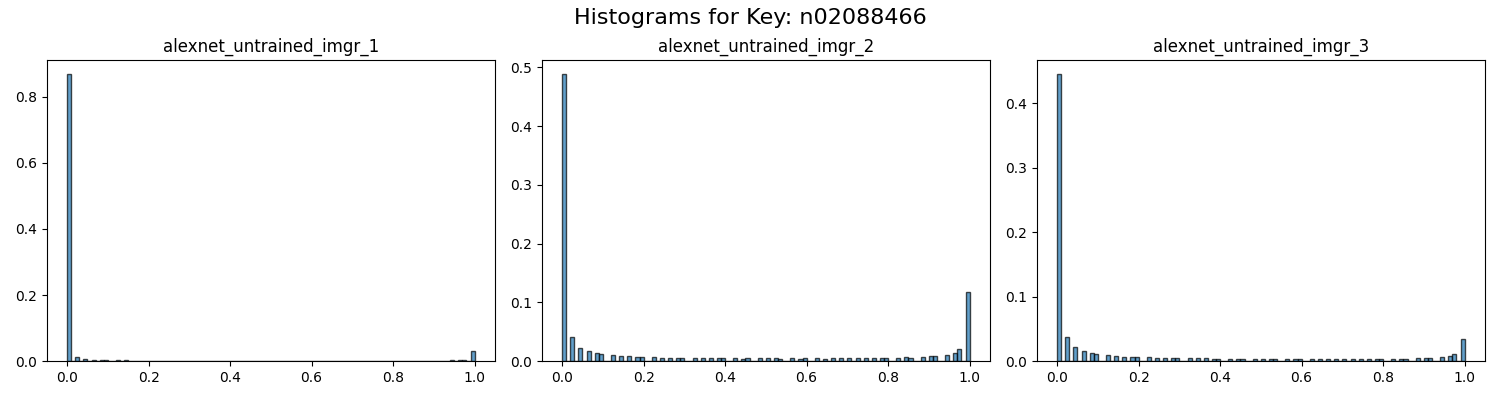
\includegraphics[width=\textwidth]{alexnet_untrained_imgr_n02088466.png} % first image
            
        \end{minipage}\hfill
        \begin{minipage}{\textwidth}
            \centering
            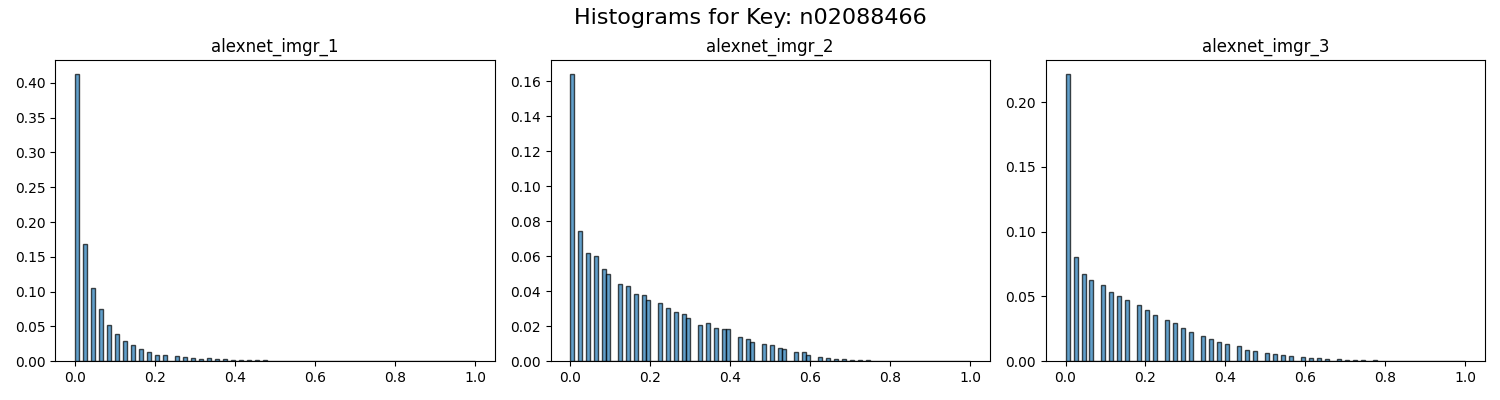
\includegraphics[width=\textwidth]{alexnet_imgr_n02088466.png} % second image
        \end{minipage}
        \begin{minipage}{\textwidth}
            \centering
            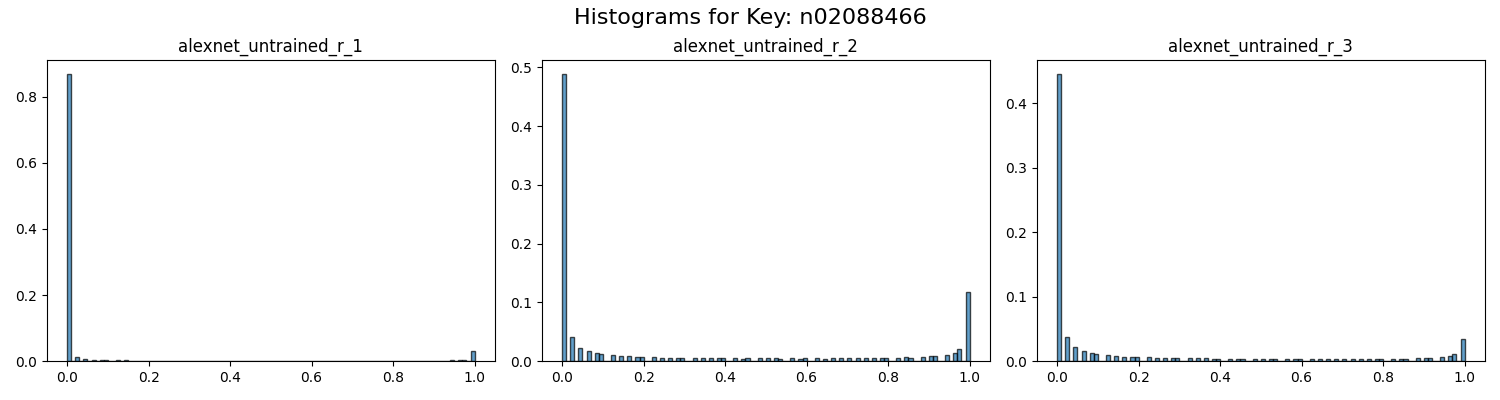
\includegraphics[width=\textwidth]{alexnet_untrained_r_n02088466.png} % first image
            
        \end{minipage}\hfill
        \begin{minipage}{\textwidth}
            \centering
            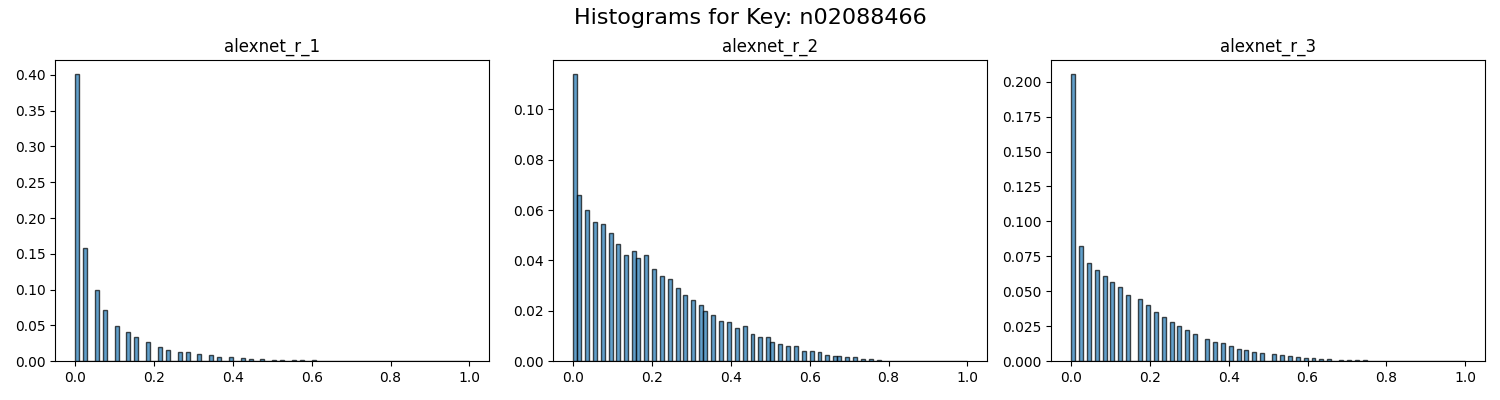
\includegraphics[width=\textwidth]{alexnet_r_n02088466.png} % second image
        \end{minipage}
        
        \caption{Frequencies of the significant neuron-weight activation proportions for a single class top: untrained on imagenet, second: trained on imagenet, third: untrained on imagenet-r, bottom: trained on imagenet-r}
        \label{fig:frequency_neuron_weight1}
    \end{figure}
    
    \begin{figure}[H]
        \centering
        \begin{minipage}{\textwidth}
            \centering
            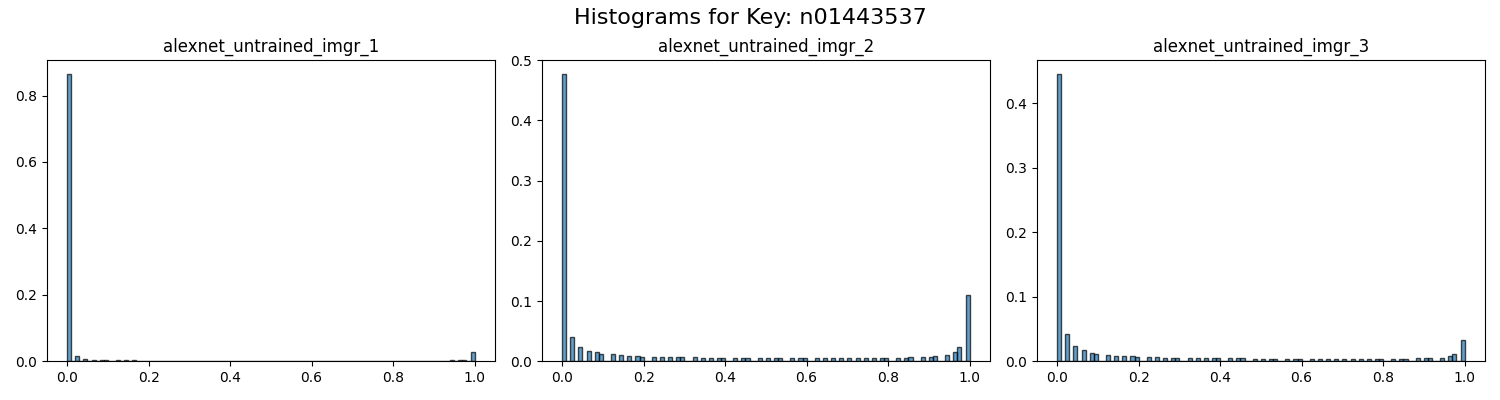
\includegraphics[width=\textwidth]{alexnet_untrained_imgr_n01443537.png} % first image
            
        \end{minipage}\hfill
        \begin{minipage}{\textwidth}
            \centering
            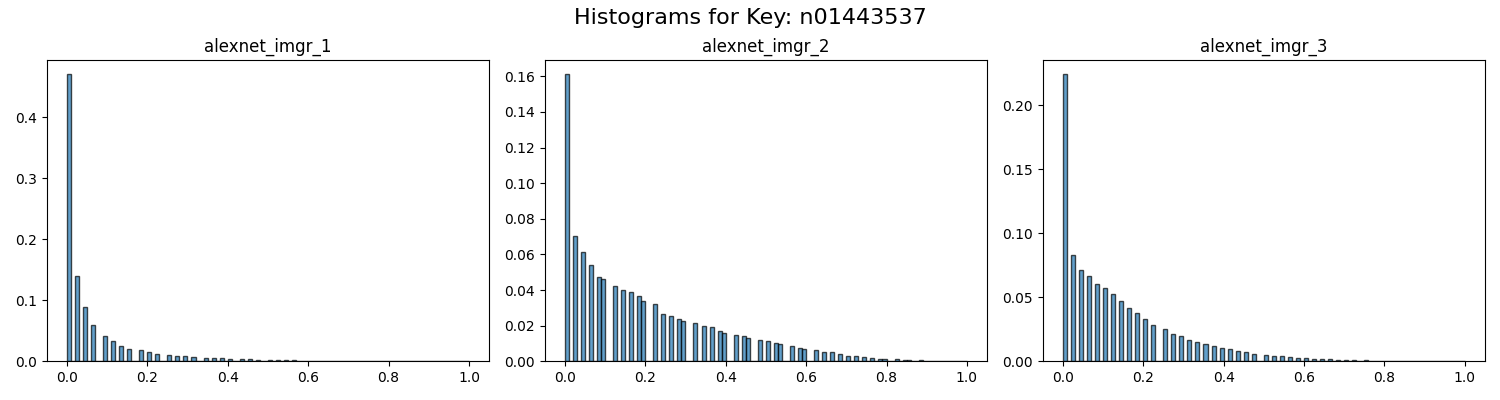
\includegraphics[width=\textwidth]{alexnet_imgr_n01443537.png} % second image
        \end{minipage}
        \begin{minipage}{\textwidth}
            \centering
            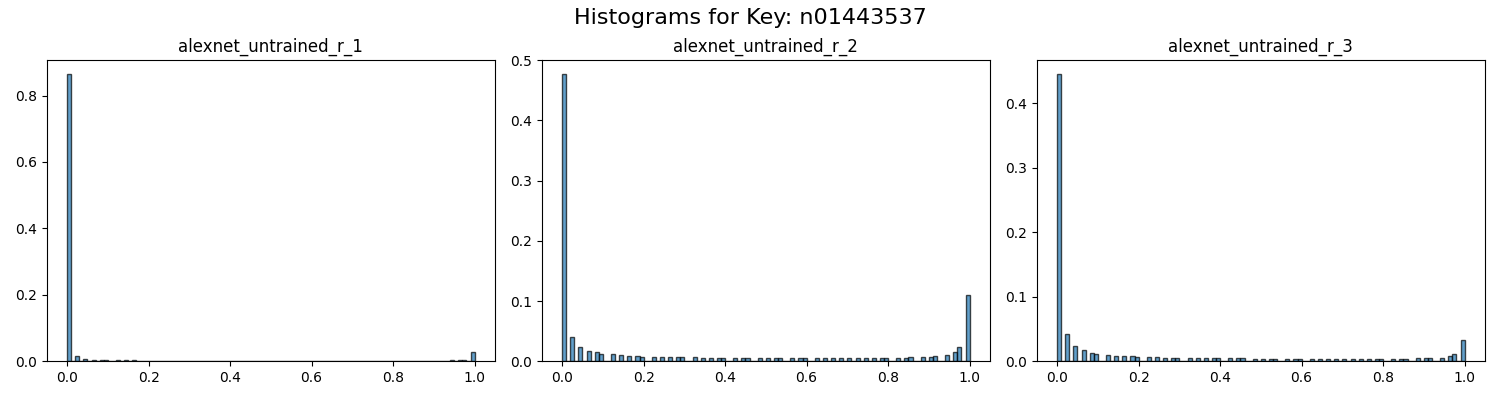
\includegraphics[width=\textwidth]{alexnet_untrained_r_n01443537.png} % first image
            
        \end{minipage}\hfill
        \begin{minipage}{\textwidth}
            \centering
            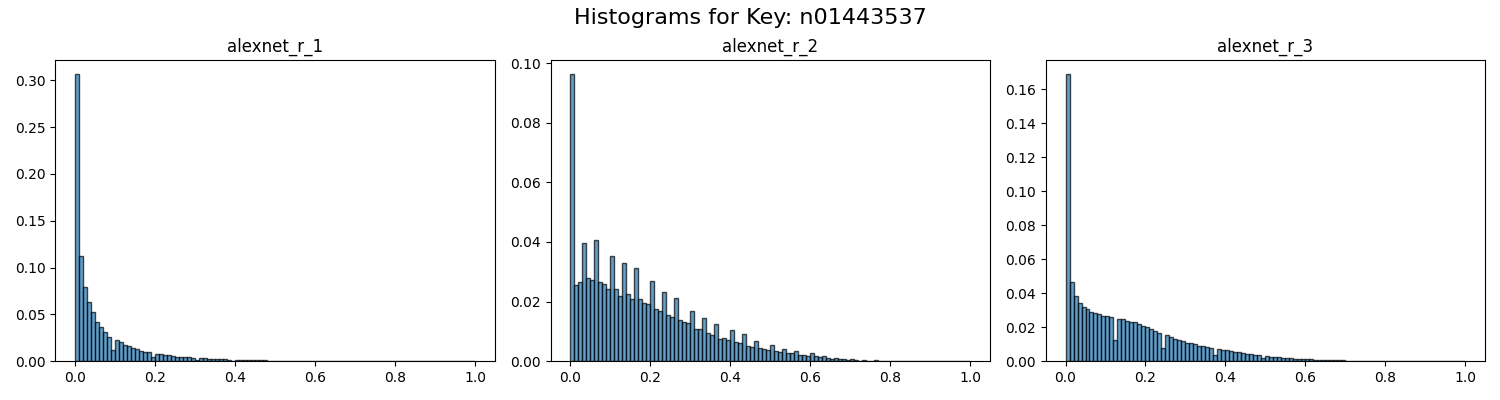
\includegraphics[width=\textwidth]{alexnet_r_n01443537.png} % second image
        \end{minipage}
        
        \caption{Frequencies of the significant neuron-weight activation proportions for a single class top: untrained on imagenet, second: trained on imagenet, third: untrained on imagenet-r, bottom: trained on imagenet-r}
        \label{fig:frequency_neuron_weight2}

        Interestingly, the frequencies of different bins of activation proportions are almost identical across different layers and classes in the untrained setting. In the trained setting, the number of 'stray' activations is much larger for the OOD case as expected, which leads to a more gradual drop-off. In the case of class n01443537, the drop is also highly irregular. The broad conclusion to be drawn is that training discourages sparsity compared to a random network, but the final pattern is still sparse inside any fixed class. 
    \end{figure}
    
    
    % \section{Patterns of Activation in Neuron-Weight Interactions}

    \section{Inter-Class Divergences between distribution of Neuron Weight interactions}
        Building on the same experiment, we wanted to check both the entropies in between different classes over the activation distribution for the same layer. We also measured the same entropies at training and testing time, as well as an in and out of distribution dataset. The in-distribution dataset was the validation set for imagenet as used eariler, and the out of distribution dataset was fixed to be the imagenet-r dataset created by Hendrycks et. al.. This is a collection of stylised versions of the standard classes of imagenet such as caricatures. This dataset has 200 classes compared to the original 1000 from imagenet, and to ensure the comparison was meaningful we sampled 50 classes from the dataset uniformly at random and computed the pairwise KL divergences between pairs of classes from the imagenet validation set, between pairs of classes from the imagenet-r set and between the same classes from imagenet and imagenet-r. All of these were done at initialisation as well as after training. The results are attached below. 

    \begin{figure}[H]
        \centering
        \begin{minipage}{0.45\textwidth}
            \centering
            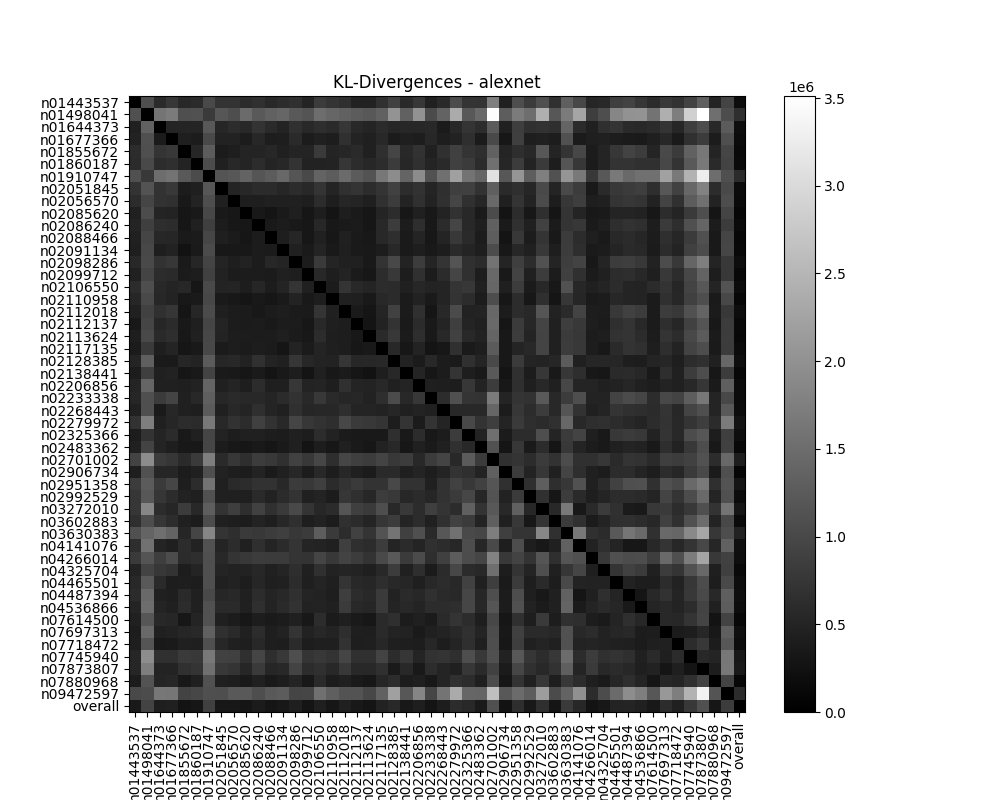
\includegraphics[width=\textwidth]{images/alexnet_kl_matrix_untrained_imgr.png} % first image
            
        \end{minipage}\hfill
        \begin{minipage}{0.45\textwidth}
            \centering
            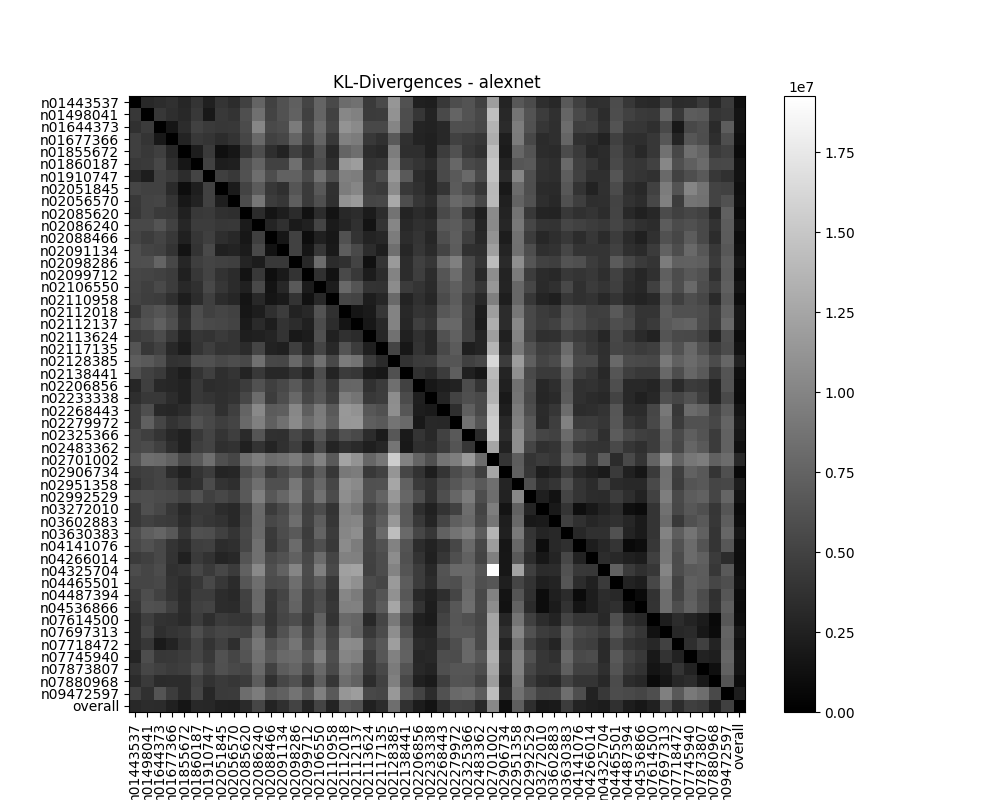
\includegraphics[width=\textwidth]{images/alexnet_kl_matrix_imgr.png} % second image
        \end{minipage}
        \begin{minipage}{0.45\textwidth}
            \centering
            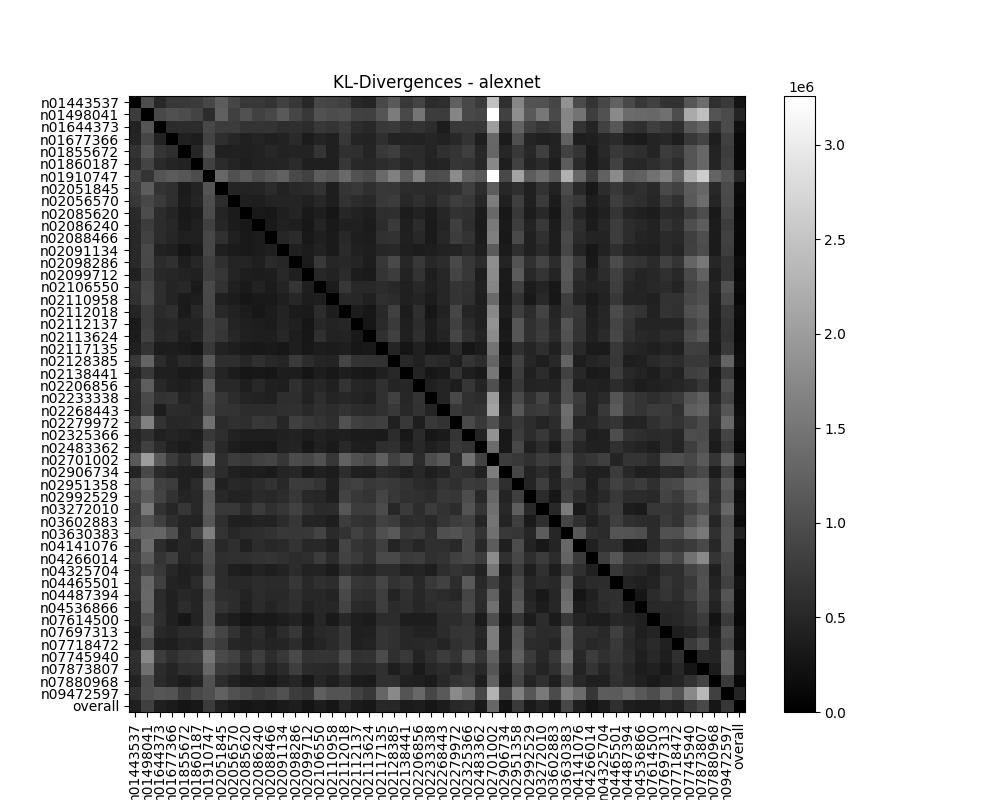
\includegraphics[width=\textwidth]{images/alexnet_kl_matrix_untrained_imgr_2.png} % first image
            
        \end{minipage}\hfill
        \begin{minipage}{0.45\textwidth}
            \centering
            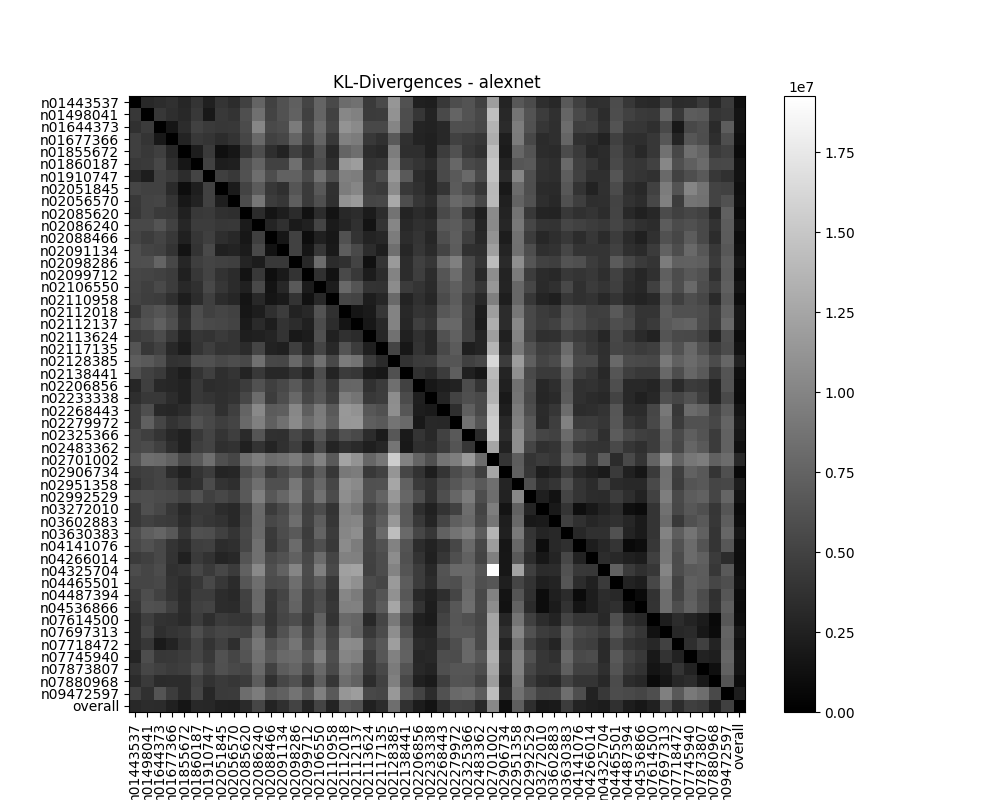
\includegraphics[width=\textwidth]{images/alexnet_kl_matrix_imgr_2.png} % second image
        \end{minipage}
        
        \caption{KL divergences between different classes for the untrained(left) and trained(right) classes of alexnet on imagenet. From top to bottom, these are the values for the distributions for the last, second last and third last layers}
        \label{fig:kl_divergences_imgr}
    \end{figure}
    
    \begin{figure}[H]
        \centering
        \begin{minipage}{0.45\textwidth}
            \centering
            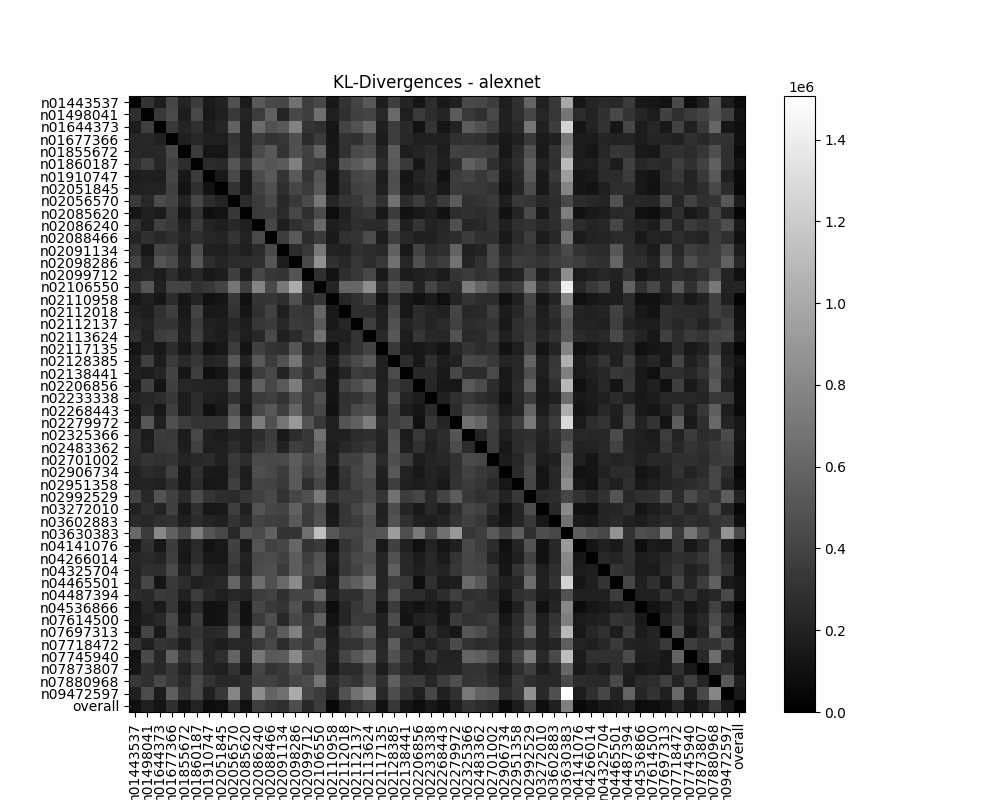
\includegraphics[width=\textwidth]{images/alexnet_kl_matrix_untrained_r.png} % first image
            
        \end{minipage}\hfill
        \begin{minipage}{0.45\textwidth}
            \centering
            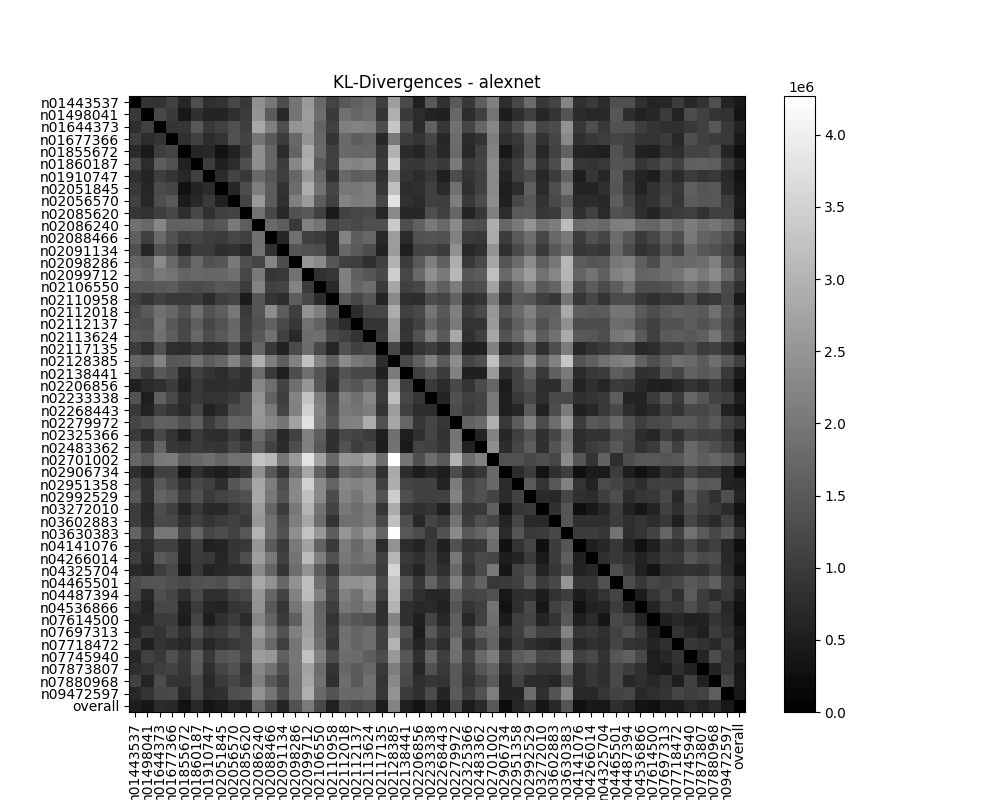
\includegraphics[width=\textwidth]{images/alexnet_kl_matrix_r.png} % second image
        \end{minipage}
        \begin{minipage}{0.45\textwidth}
            \centering
            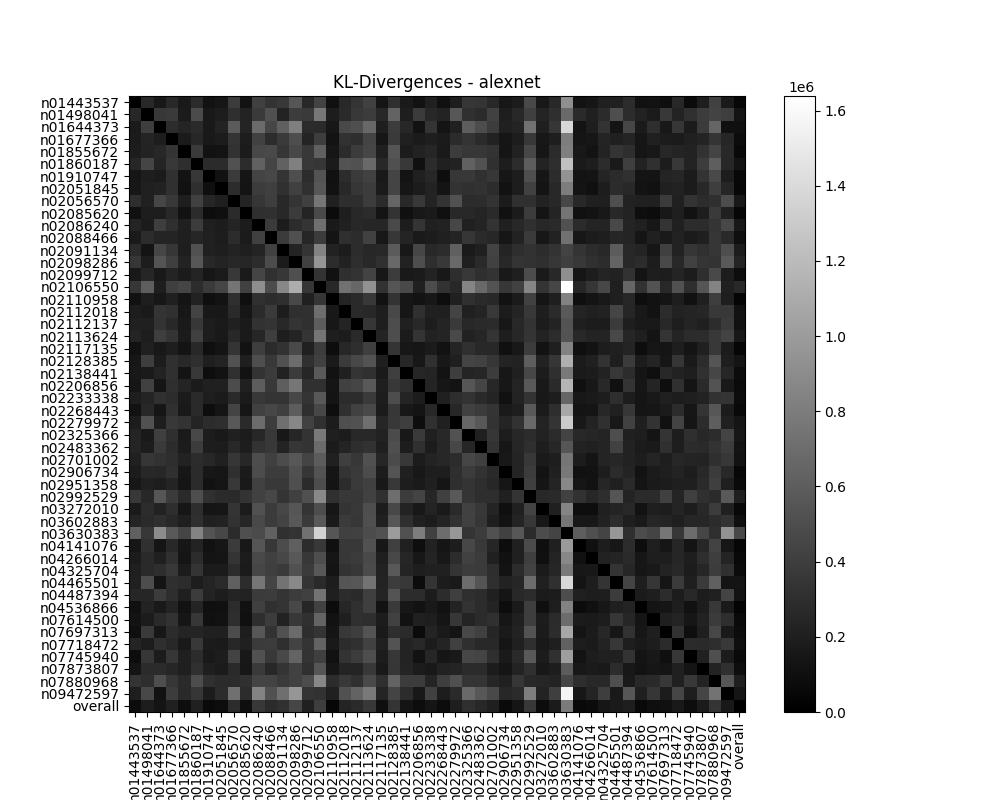
\includegraphics[width=\textwidth]{images/alexnet_kl_matrix_untrained_r_2.png} % first image
            
        \end{minipage}\hfill
        \begin{minipage}{0.45\textwidth}
            \centering
            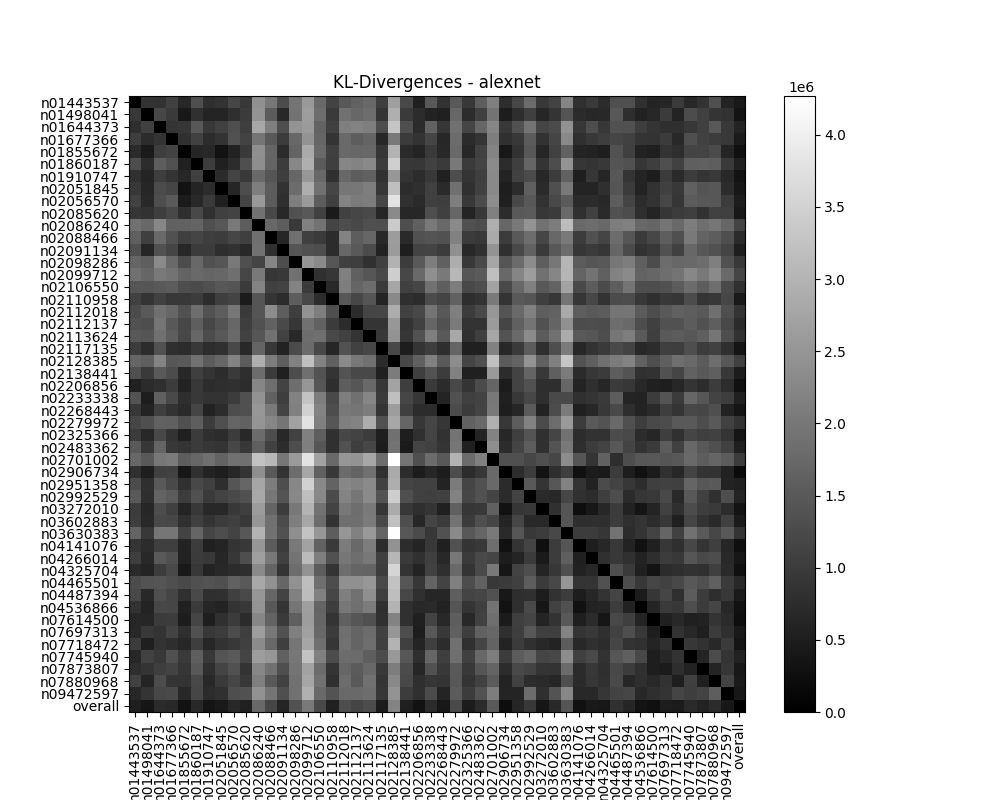
\includegraphics[width=\textwidth]{images/alexnet_kl_matrix_r_2.png} % second image
        \end{minipage}
        
        \caption{KL divergences between different classes for the untrained(left) and trained(right) classes of alexnet on imagenet-r. From top to bottom, these are the values for the distributions for the last, second last and third last layers}
        \label{fig:kl_divergences_r}

    \end{figure}
    
    The KL divergences for the distributions in the same class across the different datasets tell an interesting story. They decrease by an order of magnitude after training, suggesting that the classes do come closer together over the course of training, which suggests that the model might be 'learning' how to classify the images as compared to simply memorising the classes. They are also smaller from the OOD to the in-distribution as compared to the other way around, which would suggest that the in-distribution classes have more well-behaved distributions than the OOD class distributions which is expected. Perhaps most importantly, the classes have some separation across the 2 data distributions. This could possibly suggest one can quantify an out-of-distribution set of images using this metric.
    \begin{figure}[H]
        \centering
        \begin{minipage}{0.45\textwidth}
            \centering
            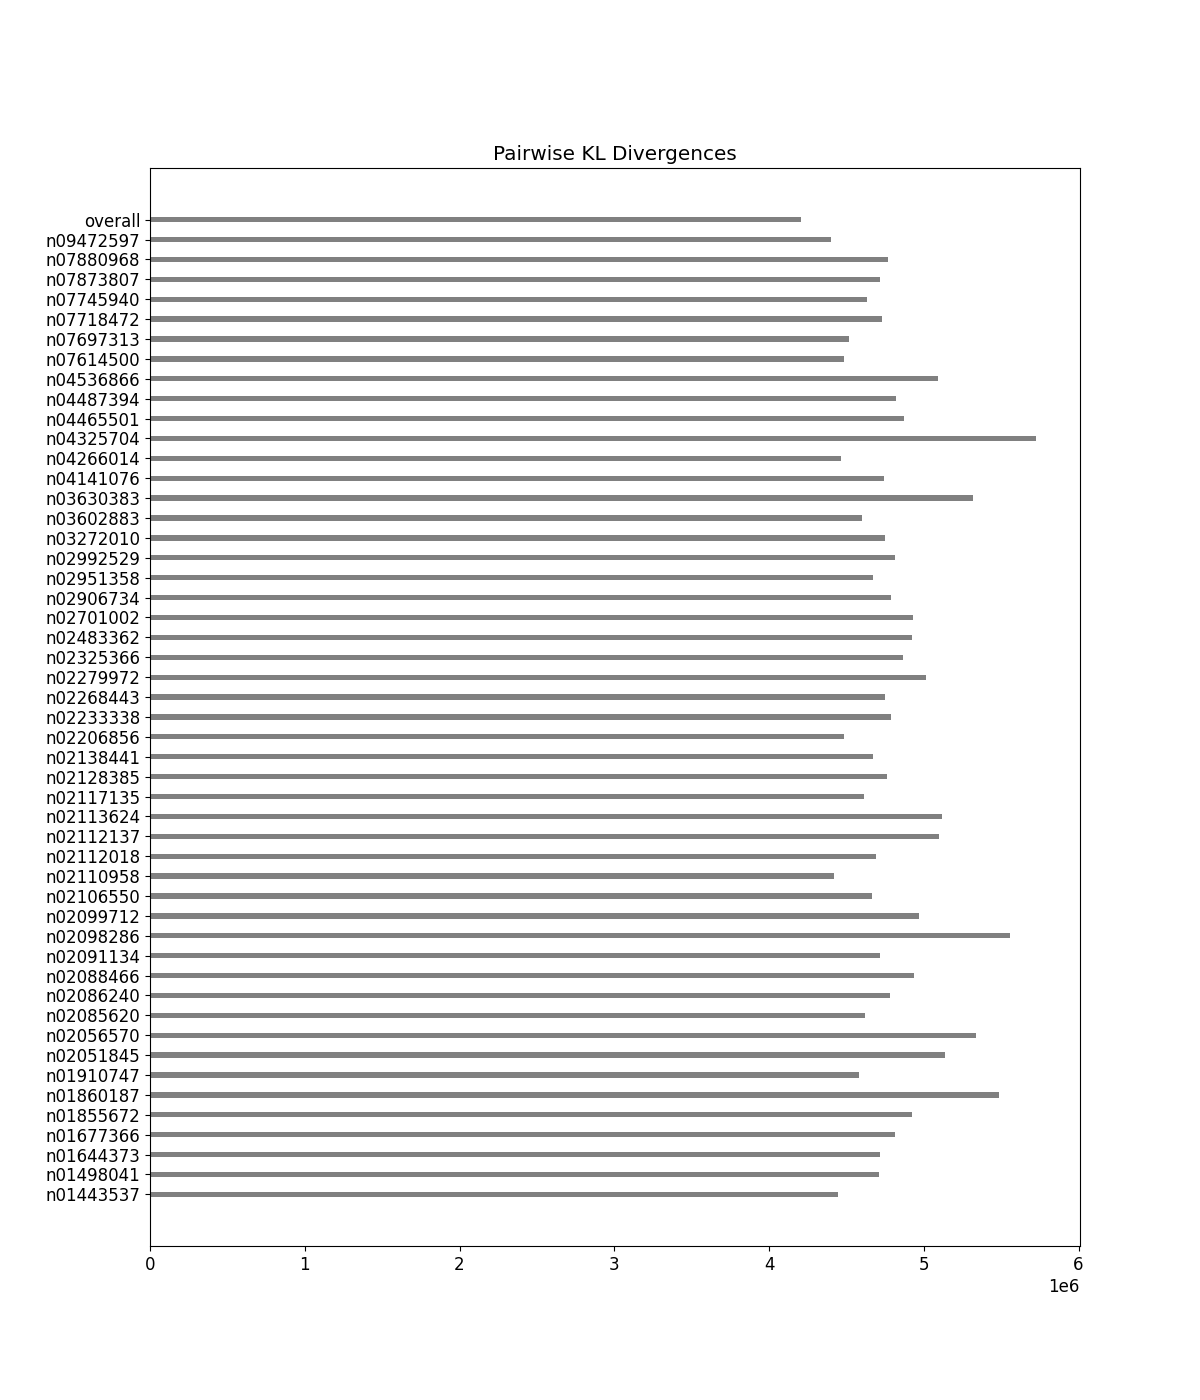
\includegraphics[width=\textwidth]{cross_imagenet_imgr_r_untrained/alexnet_kl_div_a_to_bpairwise.png} % first image
            
        \end{minipage}\hfill
        \begin{minipage}{0.45\textwidth}
            \centering
            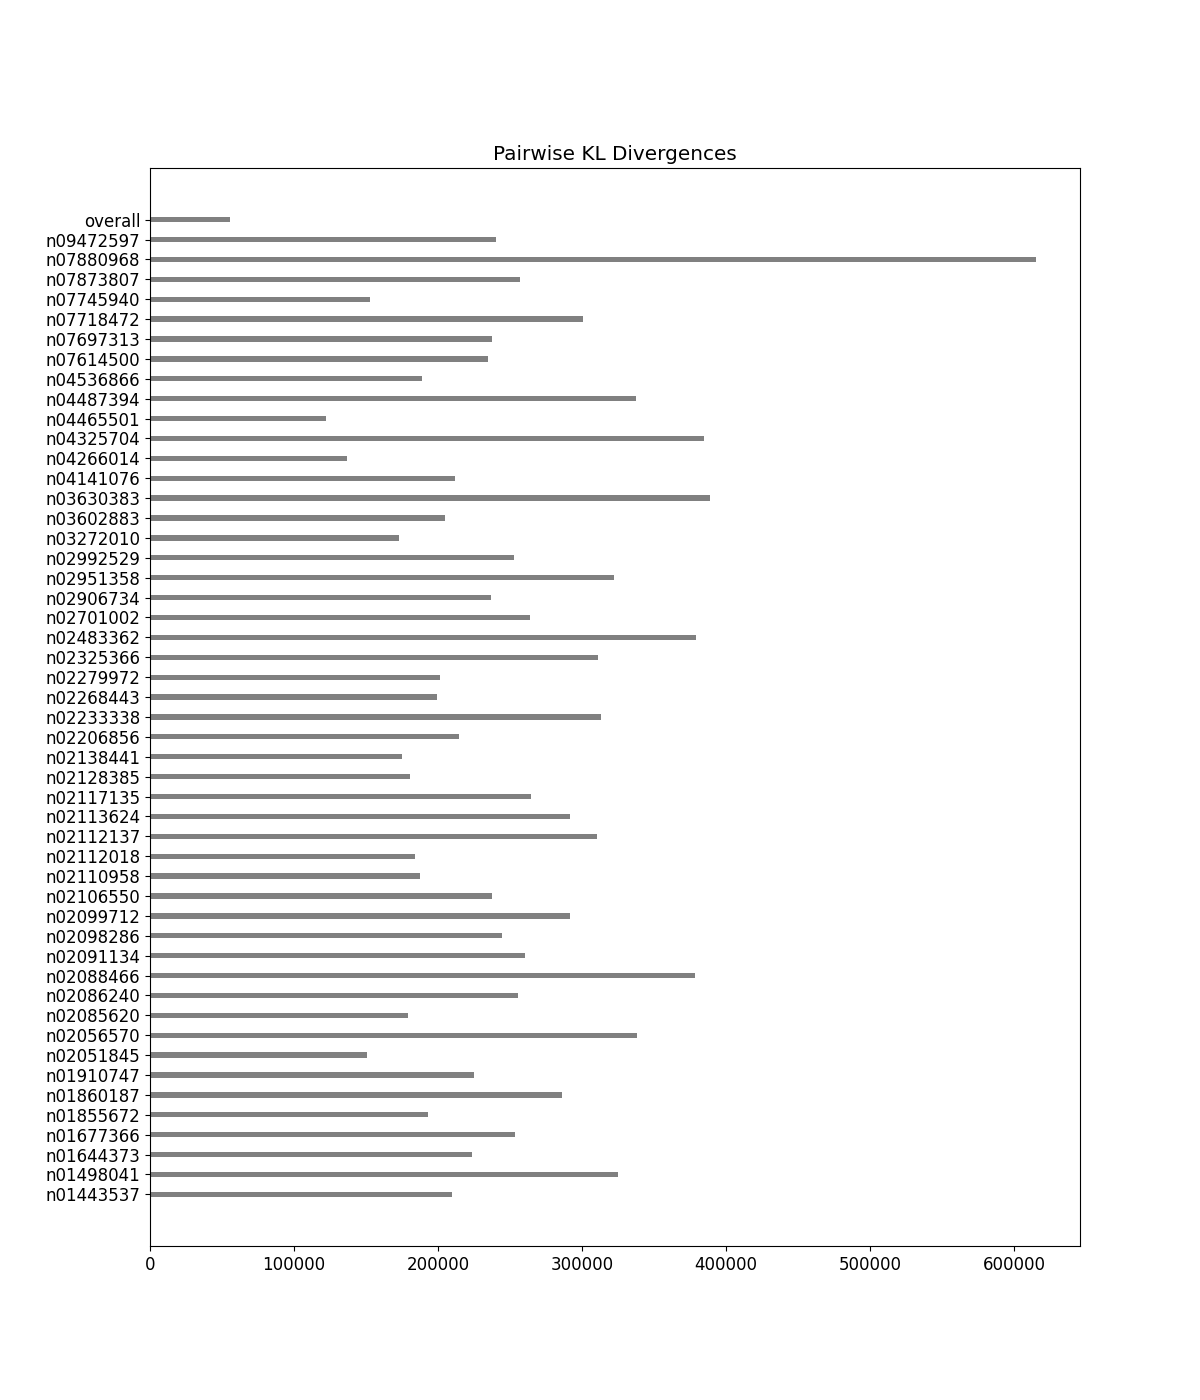
\includegraphics[width=\textwidth]{cross_imagenet_imgr_r/alexnet_kl_div_a_to_bpairwise.png} % second image
        \end{minipage}
        \begin{minipage}{0.45\textwidth}
            \centering
            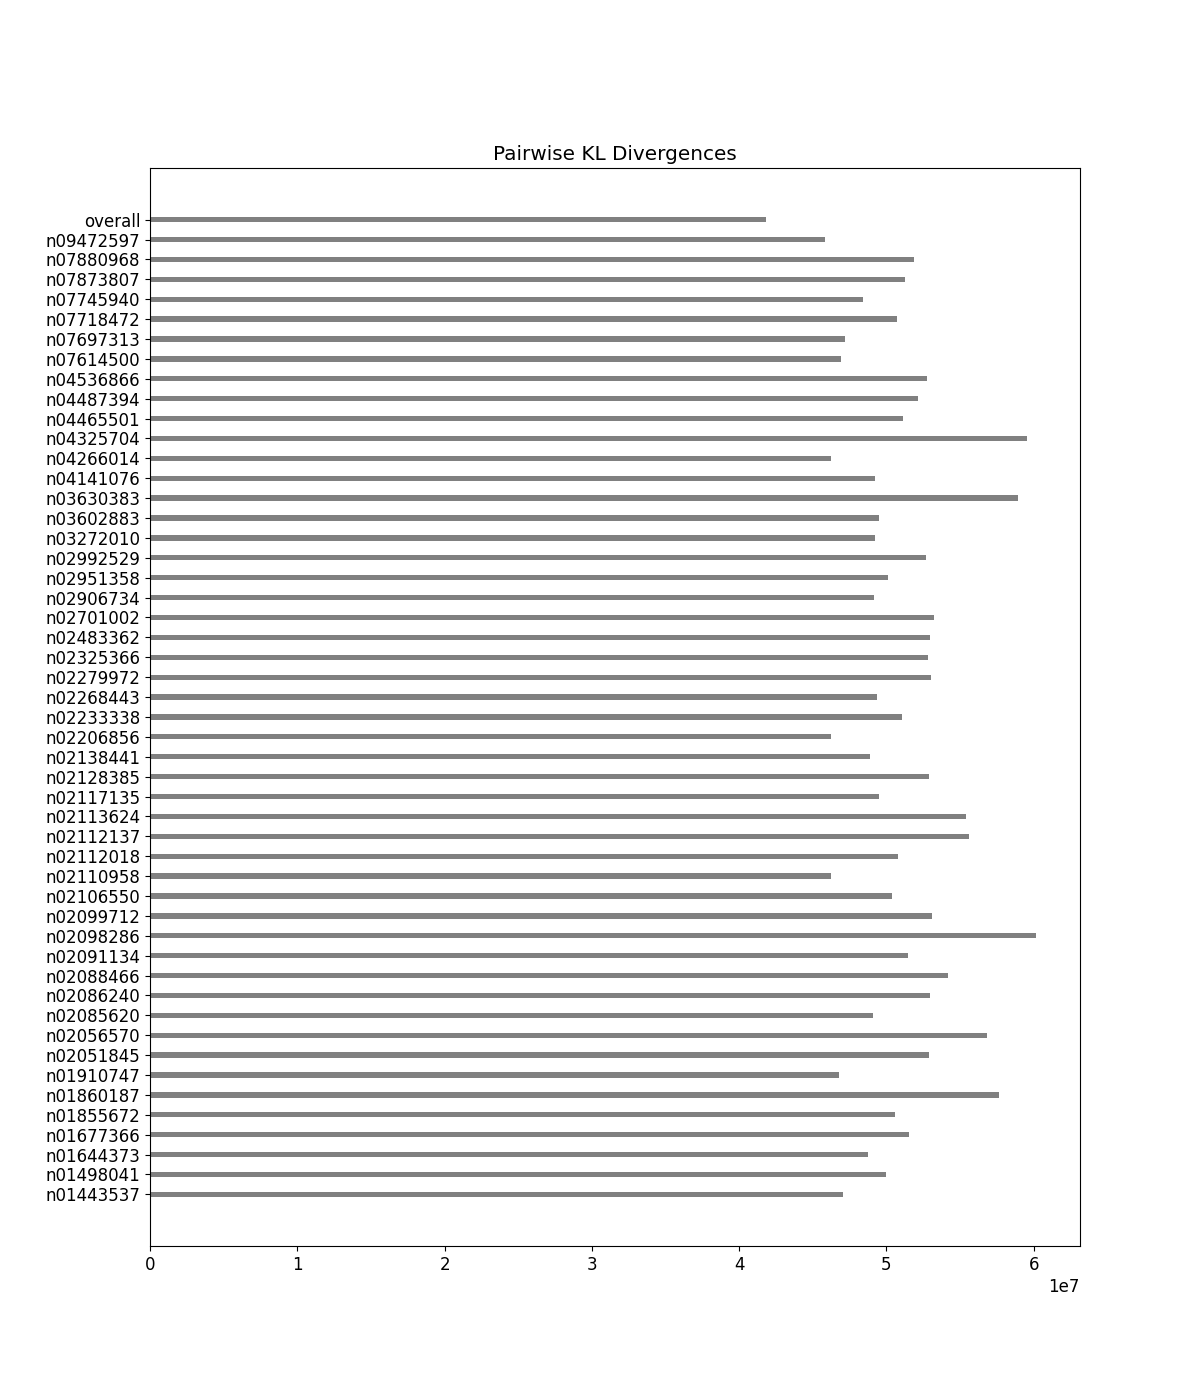
\includegraphics[width=\textwidth]{cross_imagenet_imgr_r_second_last_untrained/alexnet_kl_div_a_to_bpairwise.png} % first image
            
        \end{minipage}\hfill
        \begin{minipage}{0.45\textwidth}
            \centering
            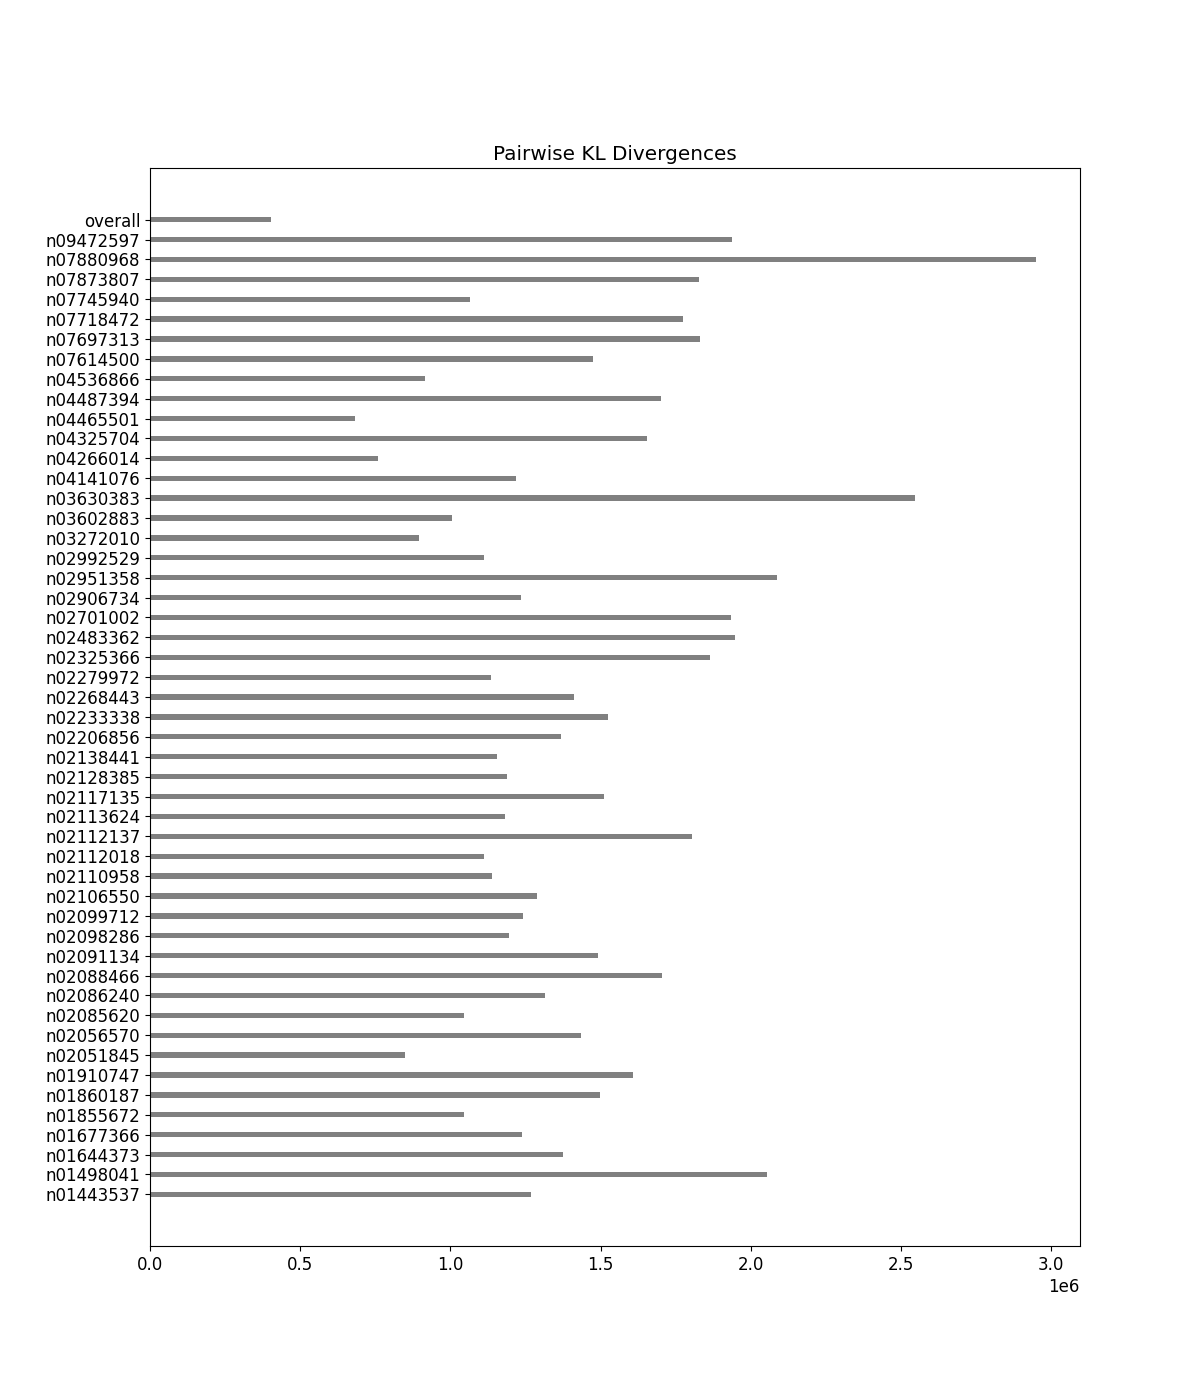
\includegraphics[width=\textwidth]{cross_imagenet_imgr_r_second_last/alexnet_kl_div_a_to_bpairwise.png} % second image
        \end{minipage}
        \begin{minipage}{0.45\textwidth}
            \centering
            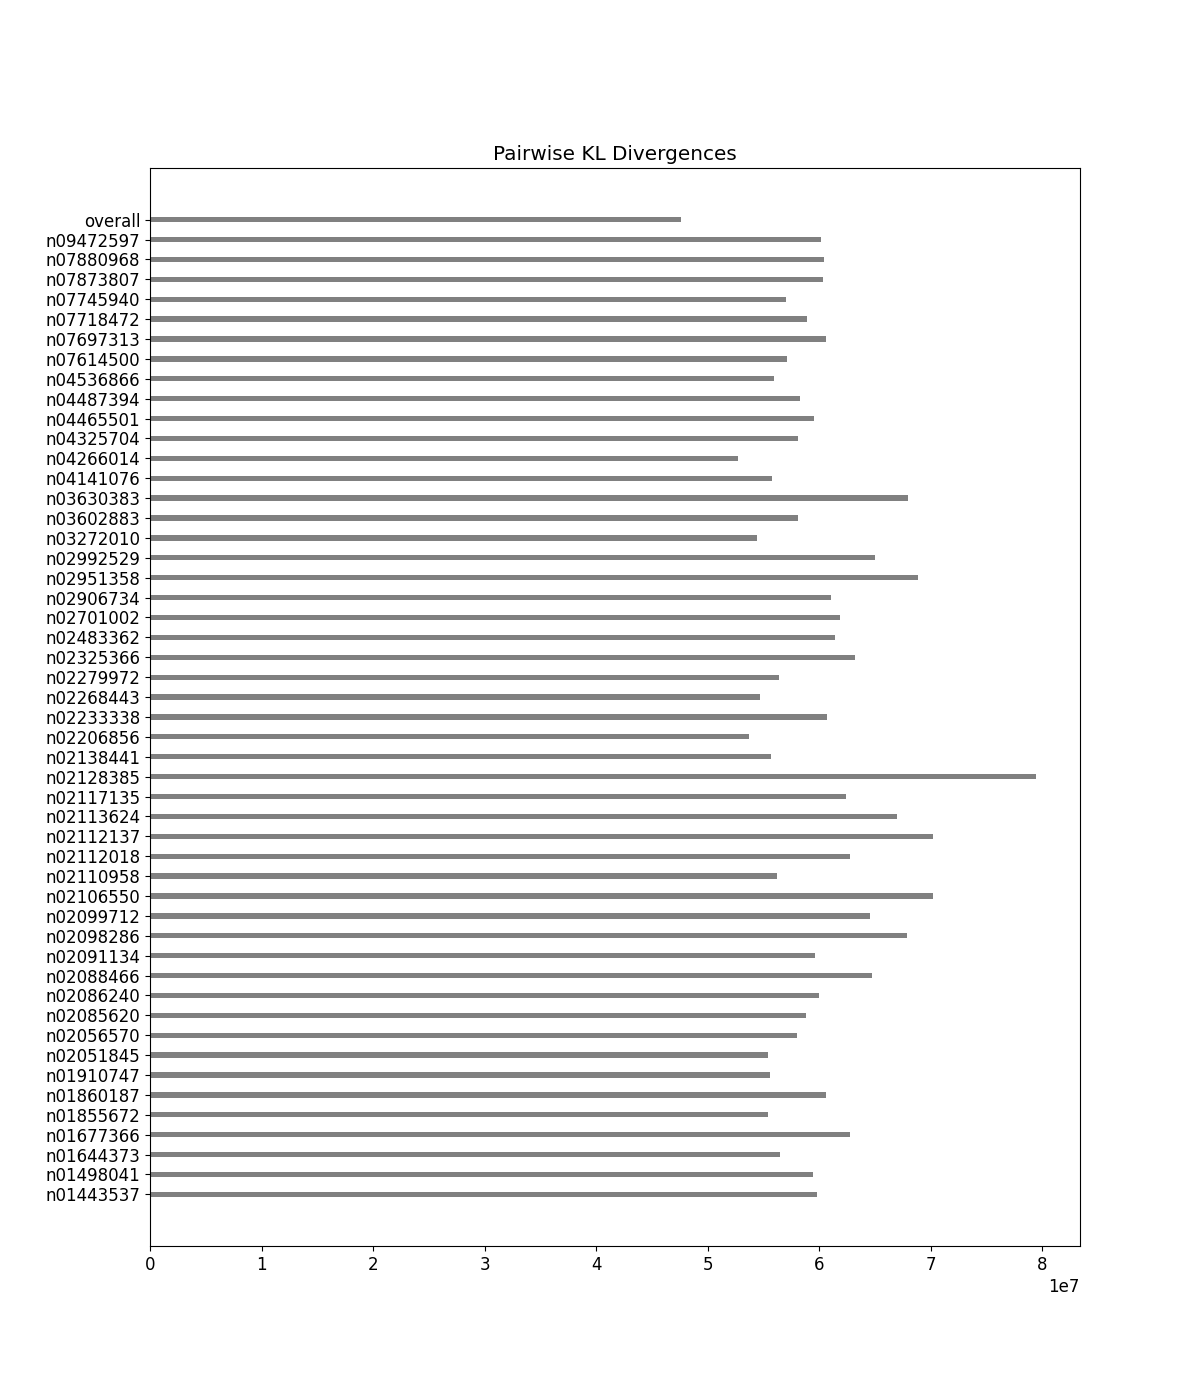
\includegraphics[width=\textwidth]{cross_imagenet_imgr_r_third_last_untrained/alexnet_kl_div_a_to_bpairwise.png} % first image
            
        \end{minipage}\hfill
        \begin{minipage}{0.45\textwidth}
            \centering
            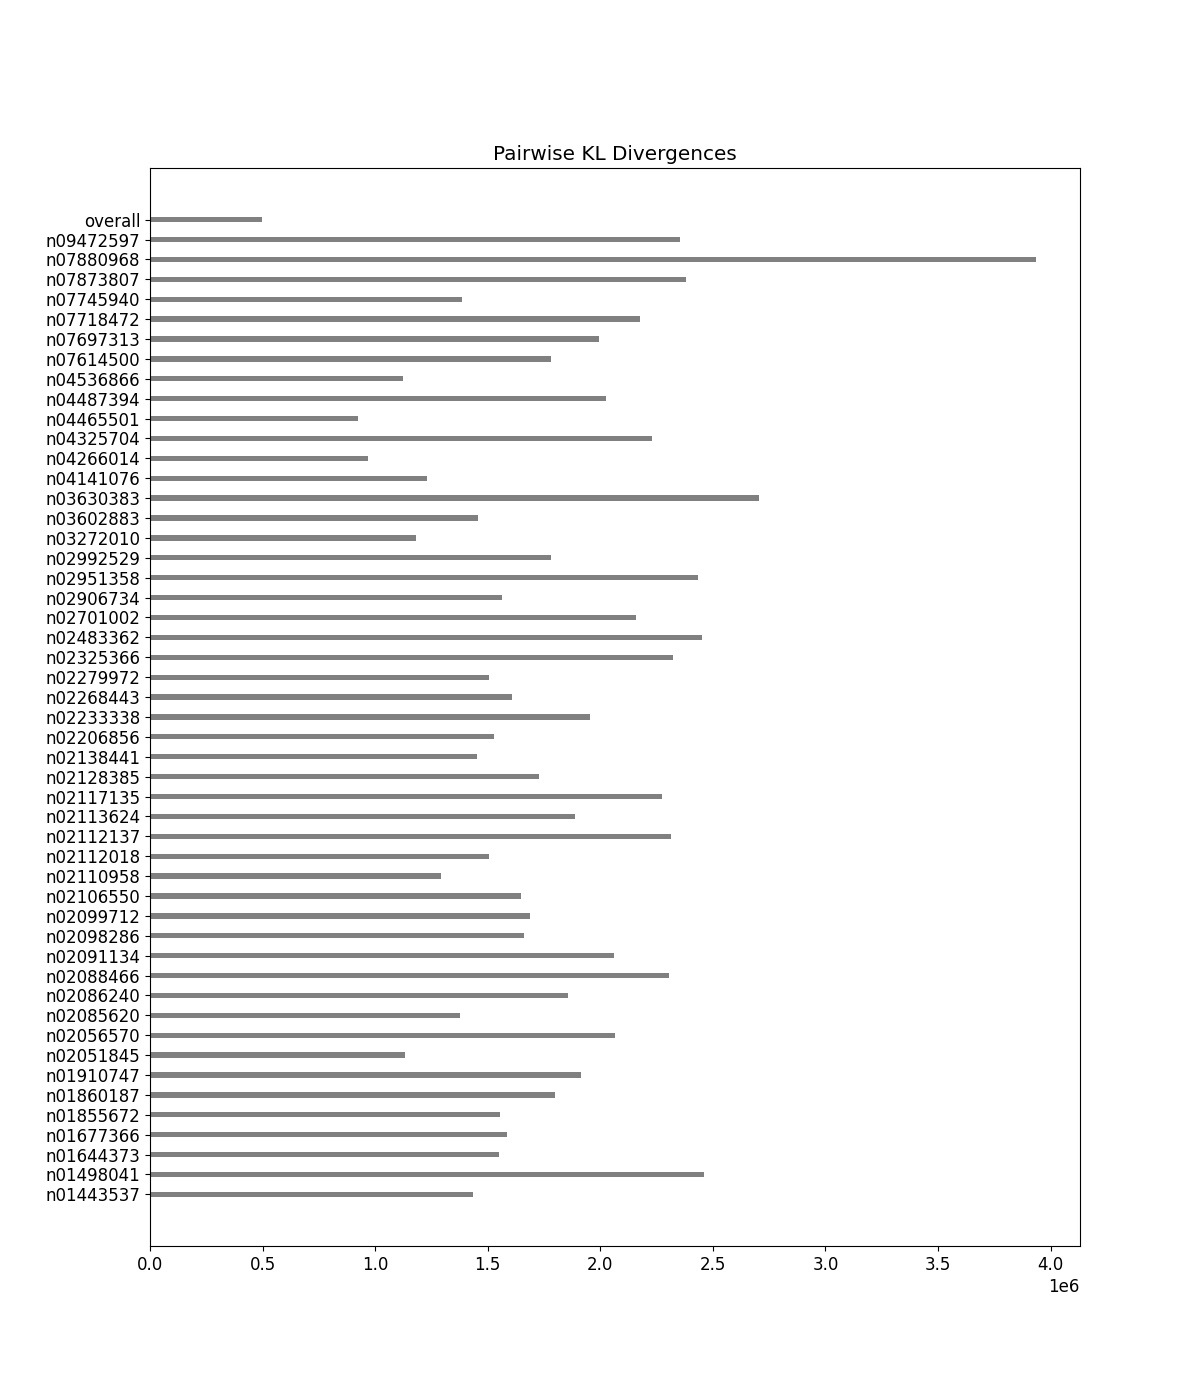
\includegraphics[width=\textwidth]{cross_imagenet_imgr_r_third_last/alexnet_kl_div_a_to_bpairwise.png} % second image
        \end{minipage}
        \caption{KL divergences from the in-distribution classes to the out of distribution classes untrained(left) and trained(right). From top to bottom, these are for the final layer, the second last layer and the third last layer}
        \label{fig:cross_kl_divergence_a_to_b}
        
    \end{figure}
    \begin{figure}[H]
        \centering
    
        \begin{minipage}{0.45\textwidth}
            \centering
            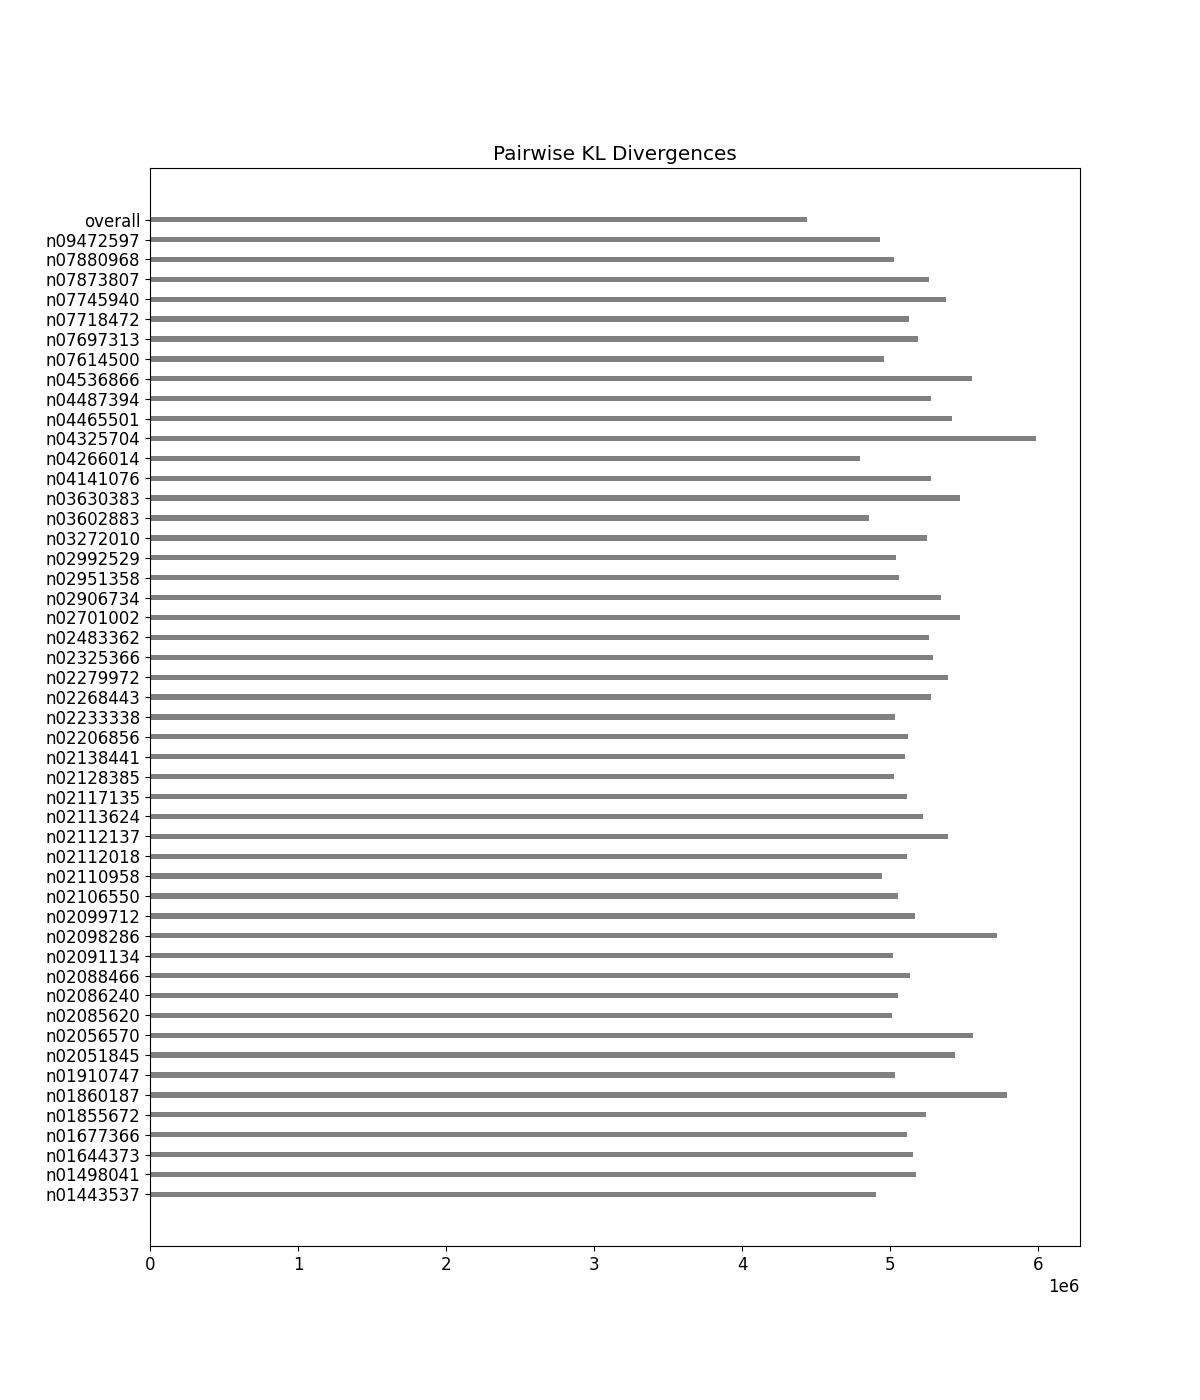
\includegraphics[width=\textwidth]{cross_imagenet_imgr_r_untrained/alexnet_kl_div_b_to_apairwise.png} % first image
            
        \end{minipage}\hfill
        \begin{minipage}{0.45\textwidth}
            \centering
            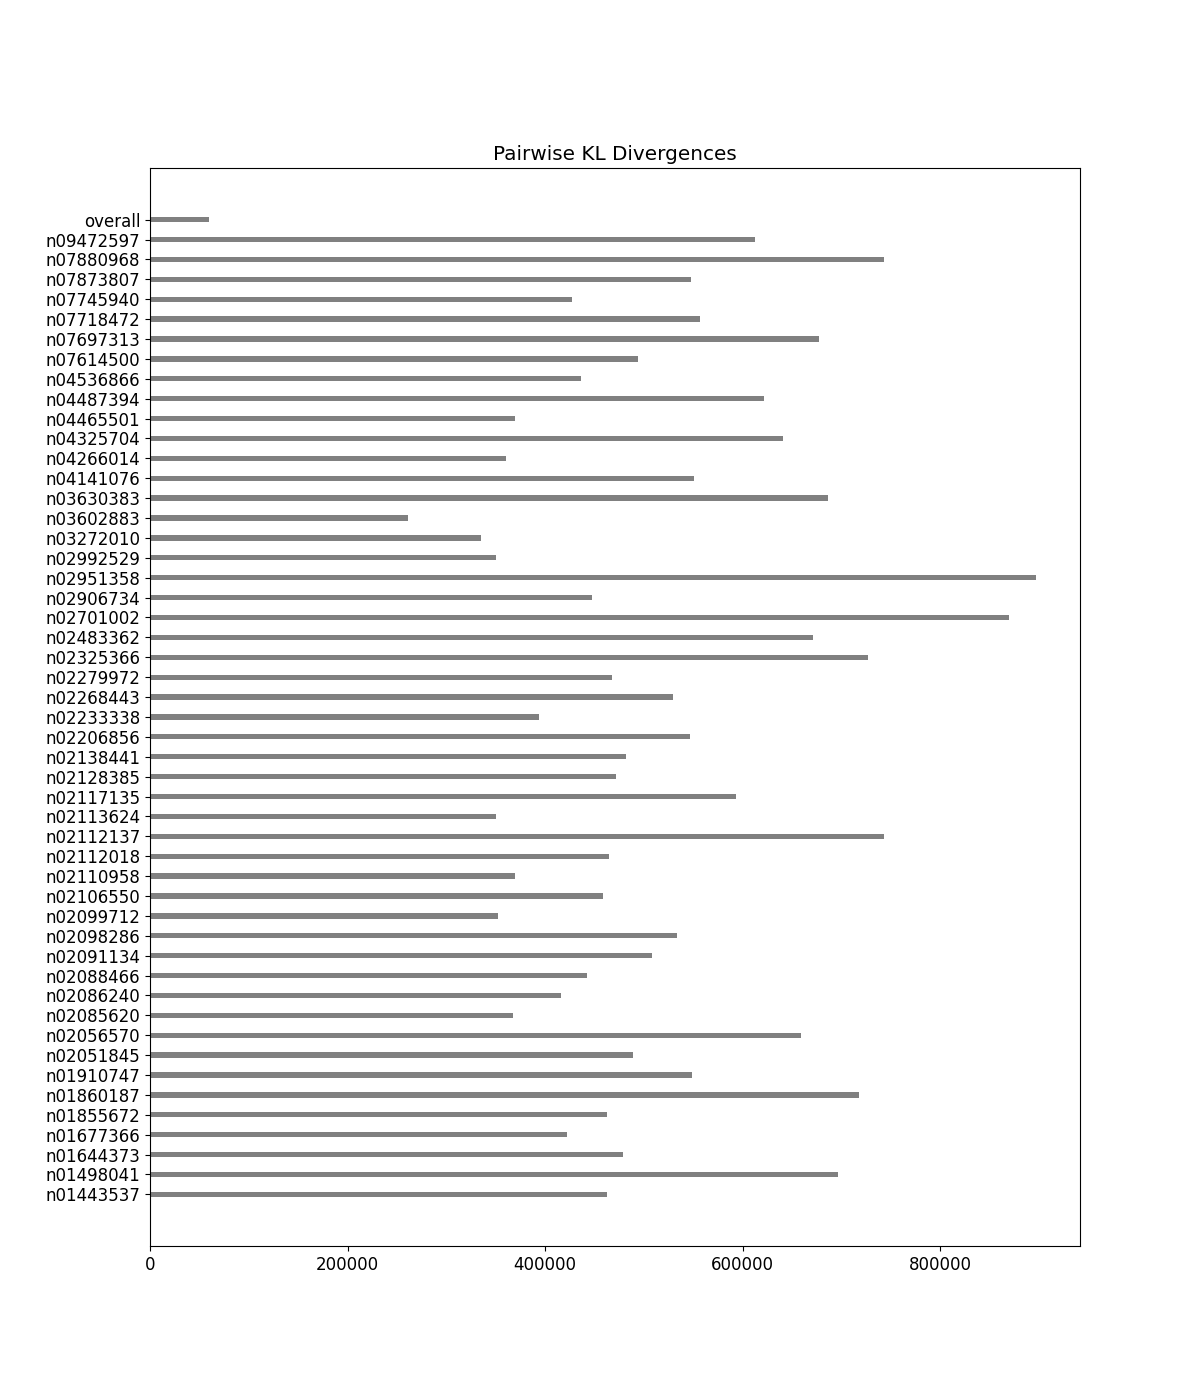
\includegraphics[width=\textwidth]{cross_imagenet_imgr_r/alexnet_kl_div_b_to_apairwise.png} % second image
        \end{minipage}
        \begin{minipage}{0.45\textwidth}
            \centering
            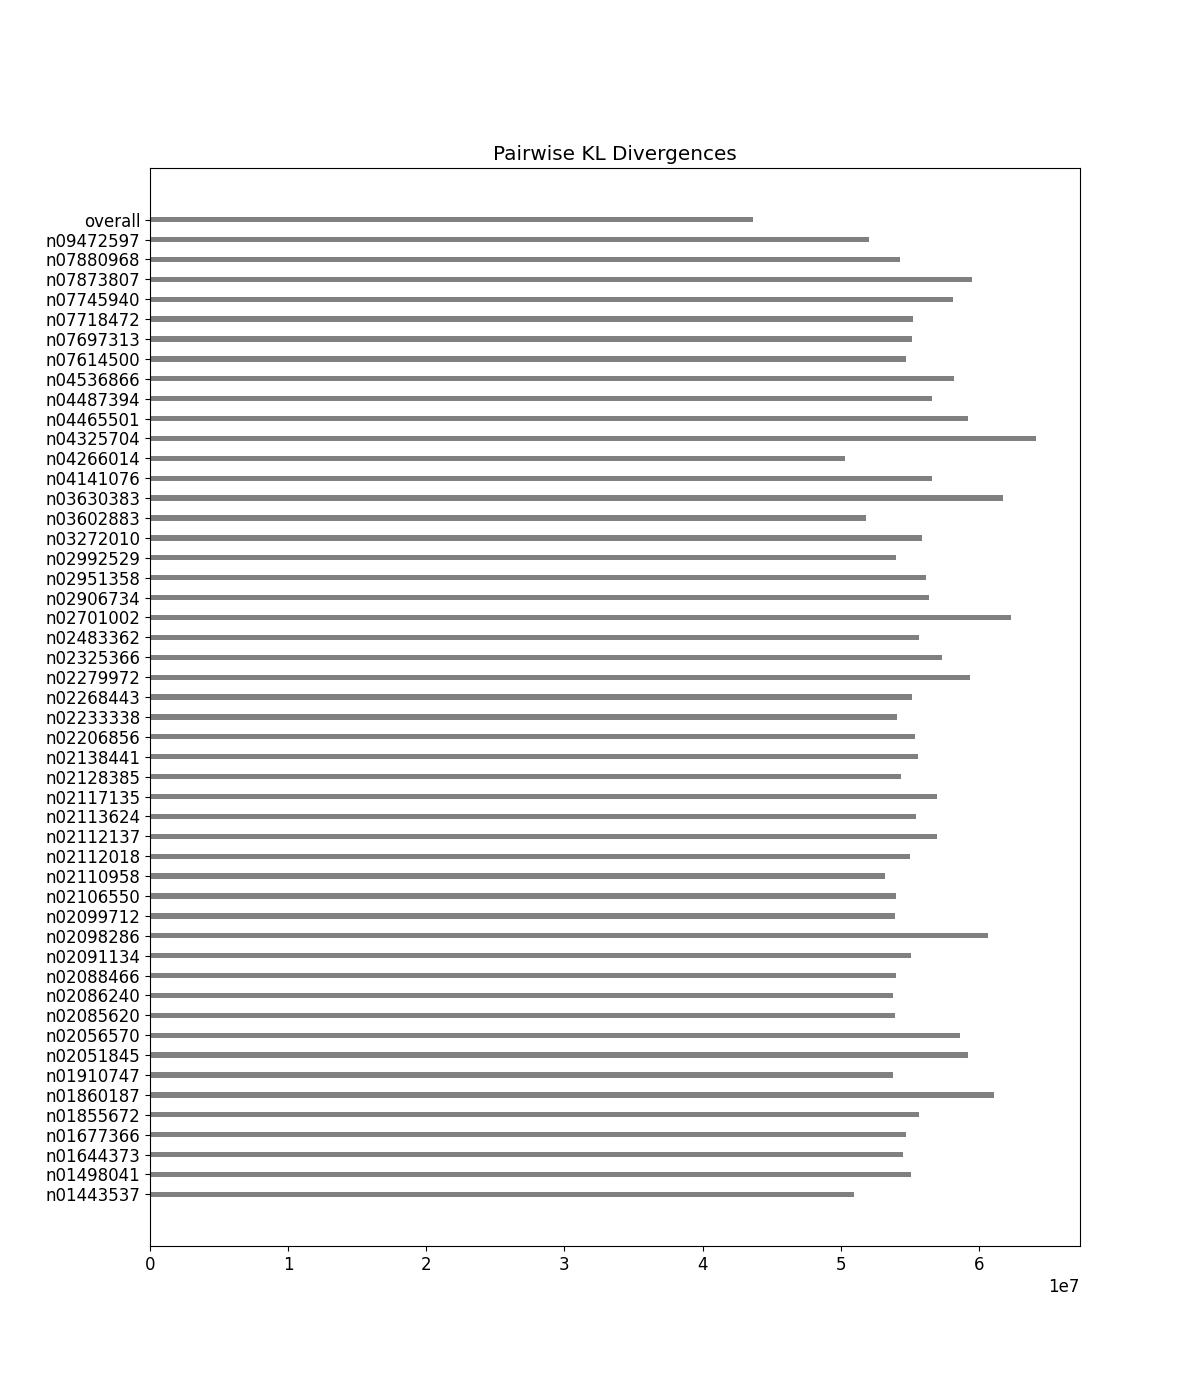
\includegraphics[width=\textwidth]{cross_imagenet_imgr_r_second_last_untrained/alexnet_kl_div_b_to_apairwise.png} % first image
            
        \end{minipage}\hfill
        \begin{minipage}{0.45\textwidth}
            \centering
            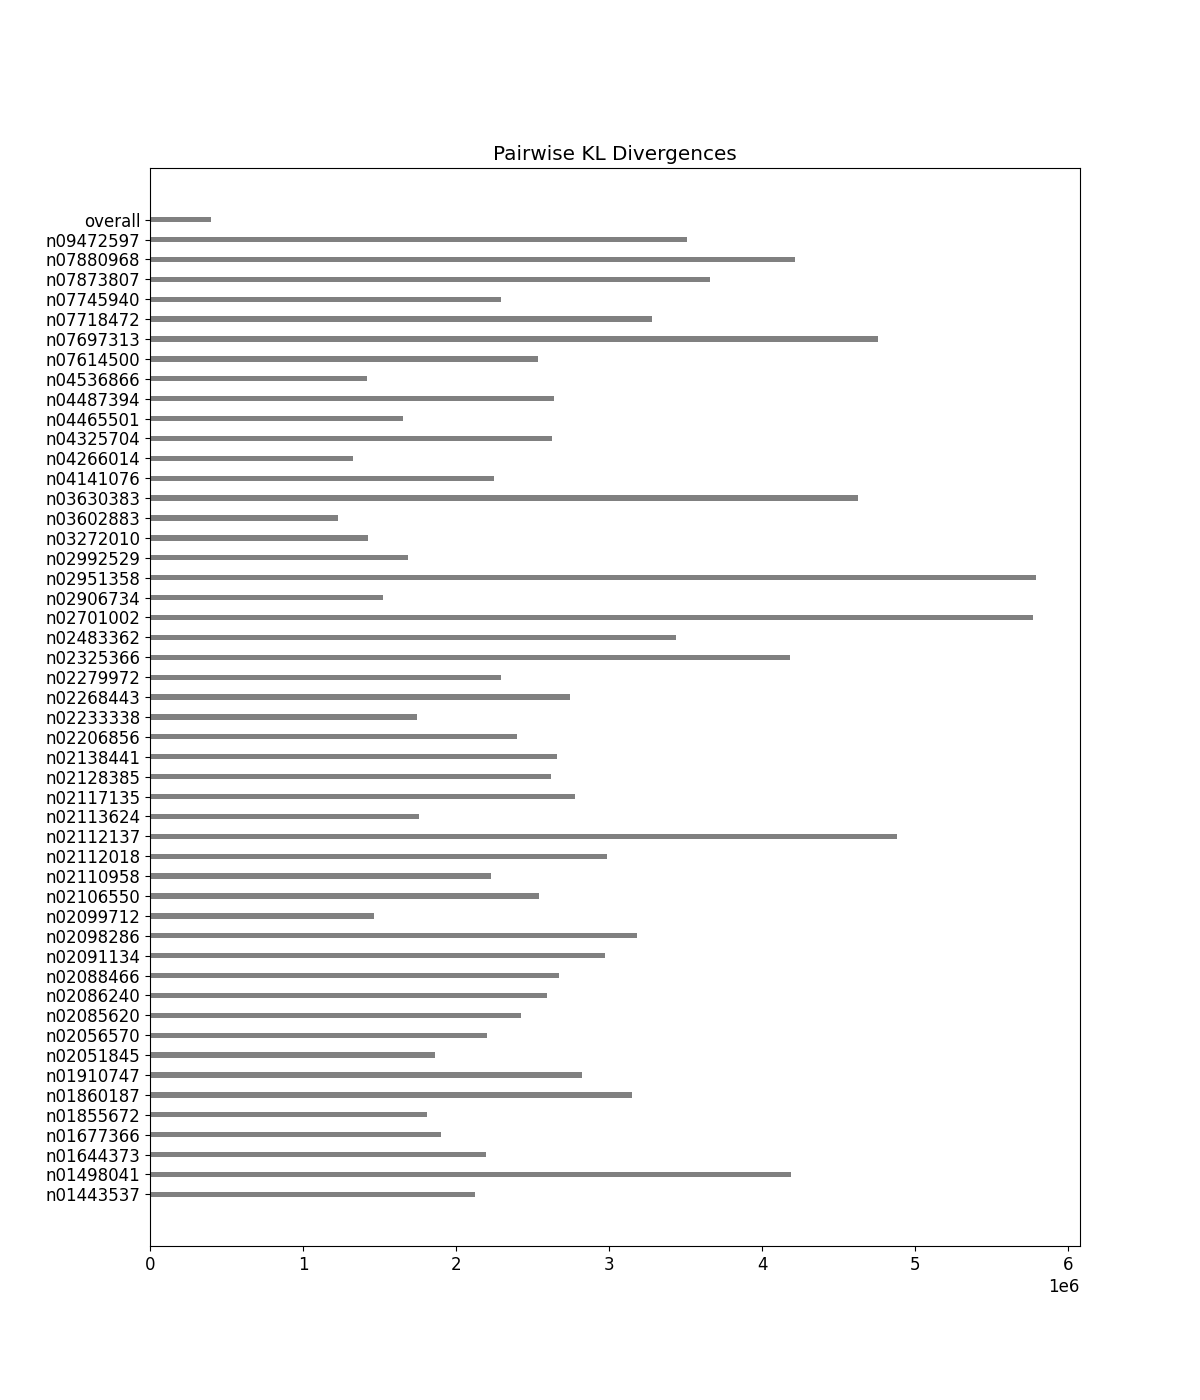
\includegraphics[width=\textwidth]{cross_imagenet_imgr_r_second_last/alexnet_kl_div_b_to_apairwise.png} % second image
        \end{minipage}
        \begin{minipage}{0.45\textwidth}
            \centering
            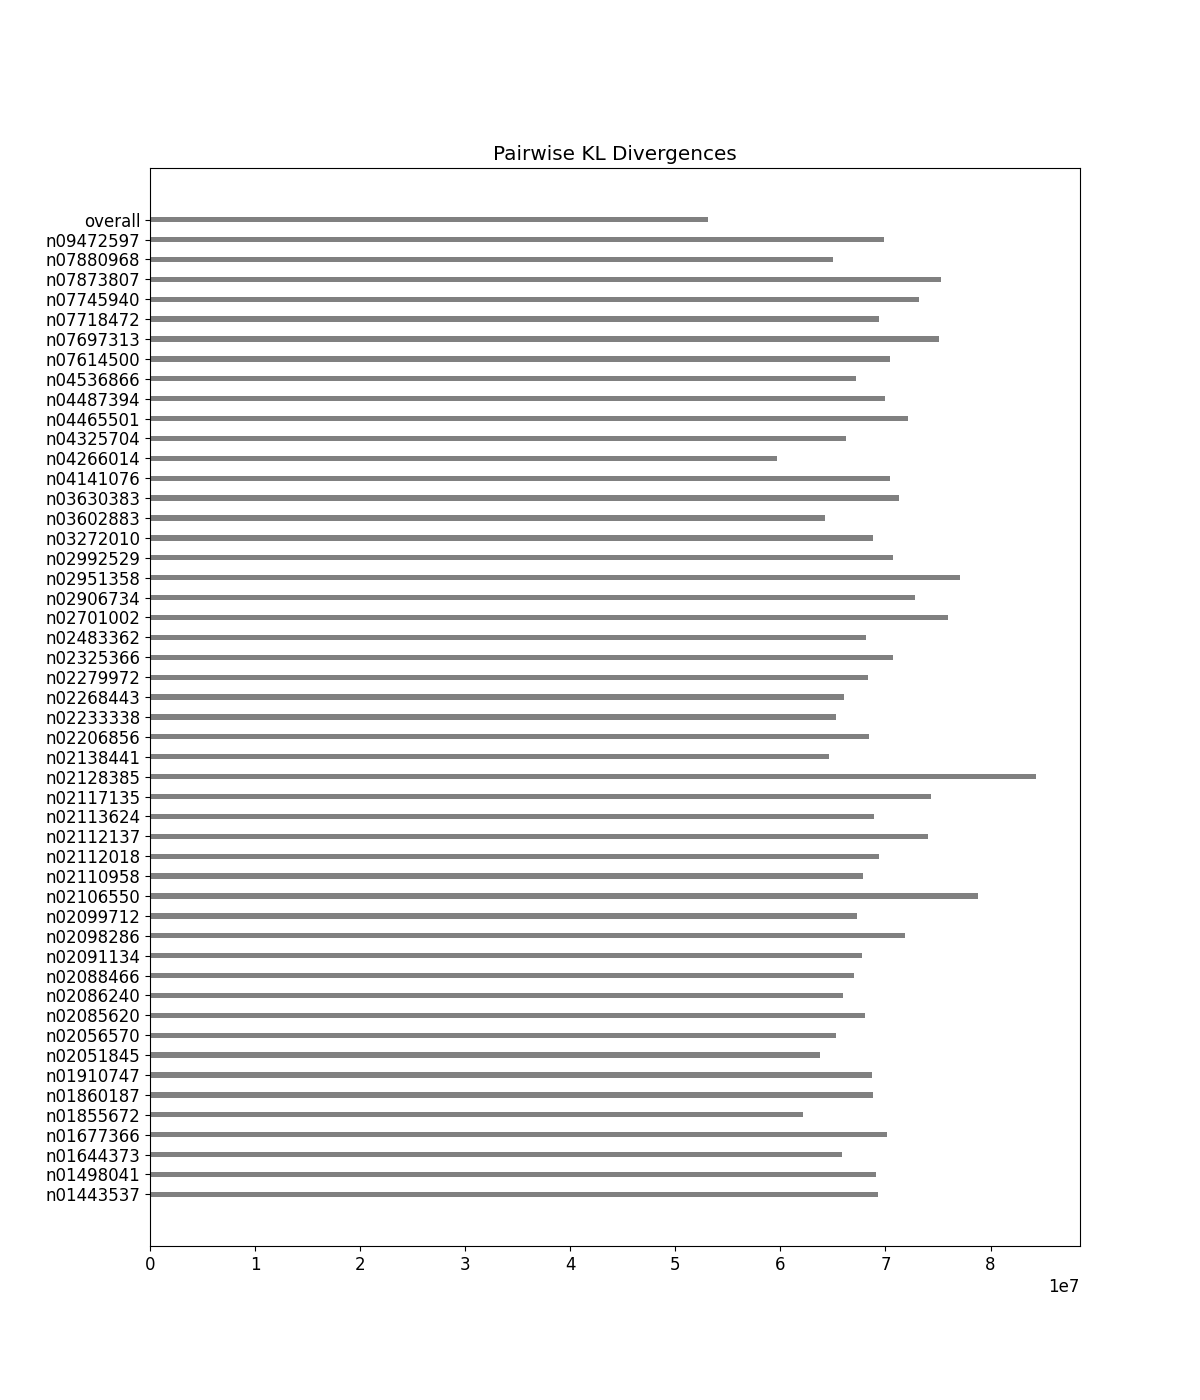
\includegraphics[width=\textwidth]{cross_imagenet_imgr_r_third_last_untrained/alexnet_kl_div_b_to_apairwise.png} % first image
            
        \end{minipage}\hfill
        \begin{minipage}{0.45\textwidth}
            \centering
            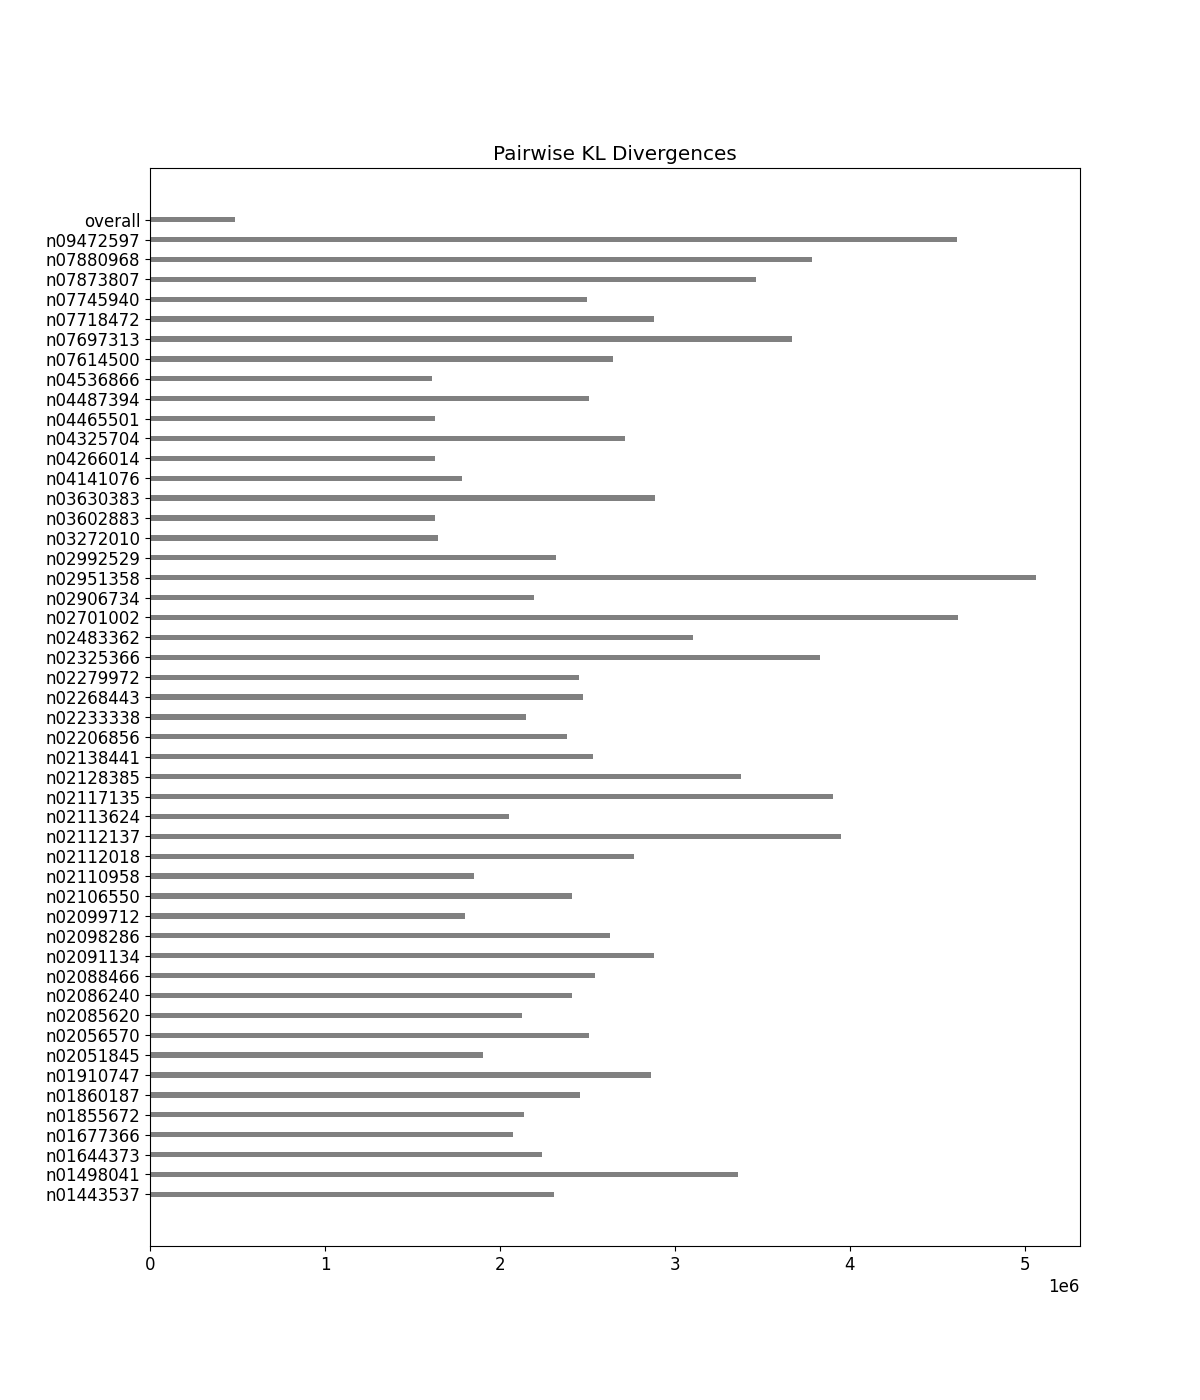
\includegraphics[width=\textwidth]{cross_imagenet_imgr_r_third_last/alexnet_kl_div_b_to_apairwise.png} % second image
        \end{minipage}
    \caption{KL divergences from the out-of-distribution classes to the in distribution classes untrained(left) and trained(right). From top to bottom, these are for the final layer, the second last layer and the third last layer}
        \label{fig:cross_kl_divergence_b_to_a}
    \end{figure}
    \section{Conclusion}
        
\end{document}
